\documentclass[a4paper 12pt]{article}
\usepackage[margin=1in]{geometry}
\usepackage{natbib}
\usepackage{epsfig}
\usepackage{amsmath}
\usepackage{amsfonts}
\usepackage{float}
\usepackage{rotating} 
\usepackage{caption}
\usepackage{subfig}
\usepackage{booktabs}
\usepackage{adjustbox}
\usepackage[table]{xcolor}
\usepackage{tabularx}
\usepackage{caption}
\usepackage{enumerate}
\usepackage{enumitem}
\captionsetup{font=footnotesize}
\newcommand{\ra}[1]{\renewcommand{\arraystretch}{#1}}
\textheight 9.0 in
\textwidth 6.5 in
%\topmargin -0.3 in
\oddsidemargin 0.0in
\renewcommand{\topfraction}{1}
\renewcommand{\bottomfraction}{1}
\renewcommand{\textfraction}{0}
\renewcommand{\floatpagefraction}{0.90}
\definecolor{TableEven}{rgb}{0.8000,0.9216,0.9490}
\usepackage{makecell}
%\usepackage{fourier} 
\numberwithin{equation}{section}
\usepackage{array}
\usepackage{titlesec}
\usepackage{sectsty}
\sectionfont{\centering}
\setcounter{secnumdepth}{4}
\usepackage{natbib}
\usepackage{siunitx}
\usepackage[toc,page]{appendix}
\usepackage{sectsty}
\usepackage{scalerel,stackengine}
\stackMath
\usepackage{graphicx}
\usepackage{amssymb}
\usepackage{xcolor}
\usepackage{hyperref}
\usepackage[normalem]{ulem} 

%\titleformat{\subsection}    
%       {\normalfont\fontfamily{phv}\fontsize{12}{17}\bfseries\itshape}{\thesubsection}{1em}{}
\subsectionfont{\normalfont\bfseries\itshape}
\subsubsectionfont{\normalfont\itshape}
%\usepackage[colorlinks,citecolor=DeepPink4,linkcolor=DarkRed, urlcolor=DarkBlue]{hyperref}
%\usepackage[svgnames]{xcolor} 
%
%\usepackage[colorlinks]{hyperref}
%\hypersetup{citecolor=DeepPink4}
%\hypersetup{linkcolor=DarkRed}
%\hypersetup{urlcolor=DarkBlue}
%\usepackage{cleveref}

%hyperlink for website will need a better option. highlights all equations etc
 \usepackage{hyperref}


\renewcommand{\baselinestretch} {2.0}
\makeatletter
\setcounter{page}{1}
\def\doublespace{\def\baselinestretch{1}\@normalsize}
\def\enddoublespace{}
\title{\bf 
}   
% \footnotemark}
\author{}
\date{}
\@addtoreset{equation}{section}
\renewcommand{\sp}{\vspace{0.2 in}}
\renewcommand{\theequation} {\arabic{section}.\arabic{equation}}
%\renewcommand{\thefigure}{\arabic{section}.\arabic{figure}}
\renewcommand{\thefootnote}{\fnsymbol{footnote}}
\newtheorem{theorem}{Theorem}
\newtheorem{lemma}{Lemma}[section]
\newtheorem{remark}{Remark}[section]
\newtheorem{corollary}{Corollary}[section]
\newtheorem{exam}{Example}[section]
\newtheorem{proposition}{Proposition}[section]

\newcommand{\Bigskip}{\vspace{0.3 in}}

\usepackage{xspace}
\newcommand{\m}{\textnormal{\sffamily m}\xspace}
\newcommand{\cm}{\textnormal{\sffamily cm}\xspace}
\newcommand{\g}{\textnormal{\sffamily g}\xspace}
\newcommand{\kg}{\textnormal{\sffamily kg}\xspace}
\newcommand{\SE}{\textnormal{\sffamily SE}\xspace}
\newcommand{\RSE}{\textnormal{\sffamily RSE}\xspace}
\newcommand{\LB}{\textnormal{\sffamily LB}\xspace}
\newcommand{\UB}{\textnormal{\sffamily UB}\xspace}


\newcommand{\mysquare}[1][black]{\small\textcolor{#1}{\ensuremath\blacksquare}}
\newcommand{\mycirc}[1][black]{\Large\textcolor{#1}{\ensuremath\bullet}}
\newcommand{\mylozenge}[1][black]{\small\textcolor{#1}{\ensuremath\blacklozenge}}
\newcommand{\mytriangle}[1][black]{\small\textcolor{#1}{\ensuremath\blacktriangle}}
\newcommand{\mydtriangle}[1][black]{\small\textcolor{#1}{\ensuremath\blacktriangledown}}
\newcommand{\mystar}[1][black]{\Large\textcolor{#1}{\ensuremath\star}} %% or \bigstar
%%%Syntax


% command for commenting
\usepackage{color}
\usepackage{ulem}
\newcommand{\ed}[1]{\textcolor{red}{#1}}
\newcommand{\nat}[1]{\textcolor{blue}{#1}}
\definecolor{darkgreen}{rgb}{0.09, 0.45, 0.27}
\newcommand{\olav}[1]{\textcolor{darkgreen}{#1}}

\makeatletter
\let\latex@xfloat=\@xfloat
\def\@xfloat #1[#2]{%
  \latex@xfloat #1[#2]%
  \def\baselinestretch{1}
  \@normalsize\normalsize
  \normalsize
}
\makeatother

\newcommand\longitude[1]{\directlua{ longitude ( \luastring{#1} ) }}


%\usepackage{lineno}
%\linenumbers

 
\begin{document}

\title{An analysis of the North Sea International Bottom Trawl Survey Data}

\maketitle


\begin{abstract}
Fish stock assessment models rely on estimates of age compositions of a fish population to provide fundamental information about the status of the stock. Abundance at age indices of fish are typically derived from estimators that use age-length keys (ALKs), which map lengths to age. However, uncertainties due to estimation of ALKs are not uncommon, and these can be included in stock assessments either by integrating the ALK estimation within the stock assessment model, or estimating the uncertainties on the derived indices outside of the model. Here, we provide estimation procedures for calculating abundance at age indices and their uncertainties of the North Sea International Bottom Trawl Survey Cod (\textit{Gadus morhua}) and Saithe (\textit{Pollachius virens}). We use ALKs with and without the assumption of constant age length structures over relatively large areas. The sensitivity of the resulting estimates with respect to the number of otoliths collected at sea is also investigated. We demonstrate how much information would be lost if the survey design was defined such that fewer otoliths were collected.


% Age length keys (ALKs) are used to map lengths to age, and we use ALKs with and without the assumption of constant age length structures over relatively large areas. All abundance at age indices are presented with variance estimates. \\
%Estimates of age compositions of fish populations are fundamental inputs to stock assessment models generally obtained from research sampling surveys and commercial catches. 
% fundamental inputs to analytical stock assessment models, and estimators based on age-length keys (ALKs) are typically used to make inference about these. 
%
%We present estimation procedures, based on ALKs, for abundance at age indices, and investigate the sensitivity of  the resulting estimates with respect to the number of otoliths sampled. The procedures presented are applied to the North Sea International Bottom Trawls Survey data for cod (\textit{Gadus morhua}) and saithe (\textit{Pollachius virens}). We demonstrate how much information would be lost if the survey design was defined such that fewer otholits were collected. 
%
%Age length keys (ALKs) are used to map lengths to age, and we use ALKs with and without the assumption of constant age length structures over relatively large areas. All abundance at age indices are presented with variance estimates. \\
%%In this research we present an approach for optimising sampling effort of the North Sea International Bottom Trawl Survey Data. 
%In this research we present estimation procedures for calculating abundance at age indices, and investigate the sensitivity of these of the resulting estimates with respect to the number of otoliths collected at sea. The procedures presented are applied to the North Sea International Bottom Trawls Survey data for cod (\textit{Gadus morhua}) and saithe (\textit{Pollachius virens}). We demonstrate how much information would be lost if the survey design was defined such that fewer otholits were collected. Age length keys (ALKs) are used to map lengths to age, and we use ALKs with and without the assumption of constant age length structures over relatively large areas. All abundance at age indices are presented with variance estimates. \\
%%In this research we present an approach for optimising sampling effort of the North Sea International Bottom Trawl Survey Data. 

\end{abstract}

% \citep{ehrhardt1997role}
\section{Introduction}
Fish stock assessments are used by fishery managers for making management decisions regarding catch quotas. The assessments provide fundamental information about the status of the stock, for instance, whether the stock is increasing and support for increased levels of harvest should be given, or whether the stock is decreasing and stricter control on harvest should be implemented. Associated with the parameters used in fish stock assessment is their uncertainty, which should not be ignored when formulating management policies \citep{ludwig1981measurement, berg2014evaluation}. This uncertainty can arise from many sources including natural variability, estimation procedures and statistical fitting. The North Sea International Bottom Trawl Survey (IBTS) data, coordinated by the International Council for the Exploration of the Sea (ICES), provides information on seasonal distribution of stocks and estimates of abundance indices and catch in numbers of fish per age-class without an assessment of the accuracy of these estimates. As stated by \citet{ludwig1981measurement} it is relevant for managers to take into account the uncertainty related to stock size when making management polices. The indices of abundance at age from IBTS  are based on data obtained from a stratified semi-random sampling approach of trawl stations,  and  it is essential to account for the sampling approach so as to produce reliable variance estimates \citep{lehtonen2004practical}. If the sampling approach is ignored, the effect on the variance  of the parameters could be substantial.  In particular, the variance could be greatly inflated  due to the clustering effect, which involves intra-cluster correlation of the variables \citep{aanes2015efficient, lehtonen2004practical}. 

There are two separate stages for generating abundance indices per age from the North Sea International Bottom Trawl Survey (IBTS) data.  The first consist of calculating indices per \textit{length} class, which are obtained by trawling in a stratified manner, sorting the catch by taxa and take biological measurement of the sorted catch. Then that knowledge is transformed to indices with respect to age. The latter part is achieved with an age-length key (ALK), which is constructed by sampling pairs of otoliths (each fish has a pair of otoliths)  in a stratified procedure from each haul and/or sub-area. To our best knowledge, there has been no research on how much the uncertainty of the abundance indices is related to these two distinct parts. The main contribution of this research is to shed light on how the indices estimates and their associated uncertainty estimates change if less effort was spent on collection of otoliths. We achieve the reduction of otoliths by mimicking a sampling procedure with less effort. We also focus on the spatial distribution of the ALK. Currently, abundance indices of IBTS are estimated using an age-length key (ALK) \citep{fridriksson1934calculation}, which is assumed to be constant over relatively large areas. We propose a design-based ALK, referred to as haul based ALK, that accounts for spatial variation. Spatial structures in the ALK have also been investigated in \citet{berg2012spatial} and  \citet{hirst2012bayesian}. 

An  overview of the  North Sea International Bottom Trawl Survey is given in Section \ref{overview}. The current estimators for ALK and catch per unit effort (CPUE) used by ICES in their database for trawl surveys (DATRAS) and our proposed ALK estimators are given in Section \ref{sec:methods}. We apply these ALK methods to two case studies in Section  \ref{sec:data}, and a discussion is given in Section \ref{sec:discussion}. The R-code for reproducing the results can be fund at github (\href{https://github.com/natoyaj/TestPackage.git}{https://github.com/natoyaj/TestPackage.git}).
 

\subsection{Overview of the North Sea International Bottom Trawl Survey}
\label{overview}
\indent The North Sea International Bottom Trawl Survey was formed in 1991, to combine the International Young Herring Survey (IYHS) and eight national surveys in the North Sea, Skagerrak and Kattegat areas. These surveys began in the 1960's, and the 1970's and 1980's, respectively. The IYHS was developed with the aim of obtaining annual recruitment indices for the combined North Sea herring (\textit{Clupea harengus}) stock \citep{ICES2012}, but yielded valuable information on other fish species such as Cod (\textit{Gadus morhua}) and haddock (\textit{Melanogrammus aeglefinus}).

\indent The North Sea IBTS began with quarterly surveys providing information on seasonal distribution of stocks, which allows changes in fish stock to be monitored and abundance of all fish species to be determined. These quarterly surveys, however became difficult to sustain as countries experienced budget cuts making it impossible to maintain high levels of research vessel effort. As such, in 1997 countries carried out a survey only twice a year; a first quarter survey (January-February) and a third quarter survey (July-September). The target species of IBTS fished from 1991-2018 includes standard pelagic species: Herring (\textit{Clupea harengus}), Sprat (\textit{Sprattus sprattus}) and Mackerel (\textit{Scomber scombrus}); and standard roundfish species: Cod (\textit{Gadus morhua}), Haddock (\textit{Melanogrammus aeglefinus}), Saithe (\textit{Pollachius virens}),  Norway Pout (\textit{Trisopterus esmarkii})  and Whiting (\textit{Merlangius merlangus}). There are also several by-catch species \citep{ICES2006Report}

Research vessels from seven nations in the first quarter (Q1) and six nations in the third quarter (Q3) are used for conducting surveys on all finfish species in the North Sea during January-February and July-August, respectively, between 1997-2018. Table \ref{countries} in Supplementary Materials \ref{secAp:areasfishedappendix} gives details of the research vessels. The sampling frame is defined by the ICES index or roundfish areas (RFA) as shown in Figure \ref{icesroufismap} numbered 1 to 10. These  roundfish areas were substratified into small strata defined by non-overlapping statistical rectangles of roughly $30 \times 30$ nautical miles ($1^{o} \  \mathrm{Longitude} \ \times  \  0.5^{o} \ \mathrm{Latitude}$), and were convenient to use for IBTS as they were already being used for fisheries management purposes. Most statistical rectangles contain a number of possible trawl hauls or tows that are deemed free of obstructions. These tows, which are referred to as   "safe tows", are taken from national databases of participating countries, DATRAS \citep{datras} or commercial fishing data. While nations are free to choose any position within a statistical rectangle to sample, tows are generally selected based on a semi-random approach from these safe tow locations. However, some nations such as Sweden and England use fixed tows, and in some cases Sweden utilizes a depth-stratified semi-random sampling design of tows \citep{ICES2018}. Sampling may be further stratified, in some statistical rectangles, due to significant changes in seabed depth which may, in turn, cause variations in the fish population. In particular, the North Sea IBTS herring, Saithe and sprat data are weighted by depth strata in the statistical rectangle \citep{ICES2013}. It is a requirement that tow locations be at least 10 nautical miles within and between statistical rectangles so as to reduce positive serial correlation, and maximize survey precision \citep{ICES2018}. Also, a target coverage of two tows is required per statistical rectangle\citep{ICES2015}, but in some statistical rectangles in the Eastern English Channel, Southern North Sea and Central North Sea intensified sampling is carried out.

The recommended standard trawling gear of the North Sea IBTS is the mulitpurpose chalut {\`a} Grande Ouverture Verticale (GOV) trawl \citep{ICES2012}, which has been used on all participating vessels since 1992, while different pelagic and bottom trawls suitable for fishing finfish species were used before 1992. Standardized trawling protocols were adopted with a towing speed of 4 knots but depending on vessel performance, tide and weather conditions the average towing speed can be at minimum 3.5 and maximum 4.5 knots. A tow duration of 30 minutes was adopted by all nations in 1999, but in the third quarter (Q3) of 2015, an experiment on tow duration was conducted in the North Sea to investigate the effect on the composition of catches. This experiment continued into the first quarter of 2016 with one participating nation \citep{ICES2016c}.  In rectangles with two hauls allocated, tow duration of one of the hauls was reduced to 15 minutes while 30 minutes tow duration was maintained for the other one. Four nations  participated in this exercise, and therefore, no mixed tow durations were planned for the Skagerrak, which is almost exclusively covered by Sweden (see Table \ref{countries} in Supplementary Materials \ref{secAp:areasfishedappendix} for all nations participating in the North Sea IBTS). The introduction of 15 minutes tows allowed to extend the survey area and resulted in a much more balanced coverage of the North Sea than in previous years. Also, there was no indication that the shorter tow were less efficient than the standard 30 minutes tows for catching larger and/or older fish in 2015 Q3. But in the first quarter of 2016 the short tows caught fewer species, the catch rates in numbers and weight were larger and the individuals caught were smaller  \citep[see][]{ICES2016c}. 

Trawling is done during the daylight hours, which are considered 15 minutes before sunrise to 15 minutes  after sunset \citep{ICES2012}. After each trawl the total catch of the different species is weighed on board and biological parameters such as length for all fish species caught are collected. Where the numbers of individuals are too large for all of them  to be measured to obtain the length distribution, a representative subsample of 100 fish is selected. A pair of otoliths are collected on board from a small fraction of all the target species from all RFAs (Figure \ref{icesroufismap}) to retrieve age reading. Table \ref{tab:otolithsTable} in Supplementary Materials \ref{secAp:otolithappendix} gives the minimum sampling levels of otoliths for the target species.
 %Denmark, Germany, Norway, and Scotland
 %This is a direct contradiction to what was found in the 2015 Q3 survey. no indication was found that the shorter tow were less efficientthan the standard 30 min tows for catching larger and/or older fish. Species richness on the other hand appeared to be slightly lower in the short than in the long tows due to the smaller fished area. They indicated neither a significant effect of tow duration on the abundance indices of NS-IBTS target species, nor on the total number of species recorded
 
%\clearpage
\begin{figure*}[h!]
\centering
\begin{tabular}{@{}ccc@{}}
\subfloat[]{\includegraphics[width=0.95\textwidth]{figures/surveyarea}} & 
\end{tabular}
\caption[]{Standard roundfish areas (RFAs) used for roundfish since 1980 and for all standard species since 1991 (left panel). RFA 10 was added in 2009. The number 1, for example, indicates ICES RFA 1. The small grey rectangles in the left panel indicates the statistical rectangles of approximately $30 \times 30$ nautical miles (these vary from ~28 nm wide in the north, to ~40 nm wide in the south of North sea) ($1^{o} \  \mathrm{Longitude} \ \times  \  0.5^{o} \ \mathrm{Latitude}$). The map in the right panel shows the Norwegian trench and shelf edge (depths 1000-1500).}
\label{icesroufismap}
\end{figure*} 

\section{\large METHODS}
\label{sec:methods}
This section gives the estimators of abundance indices. The estimators are haul-duration based and utilizes an ALK approach. We consider the ALK approach used in DATRAS and we propose two ALK estimators. The ALK used in DATRAS assumes constant  age-length structures over large areas.  As differences in age-length structures may exist over large areas, these differences do have the potential to result in a biased ALK \citep{gerritsen2006simple,kimura1977statistical}. To account for the spatial distribution we propose a design-based ALK that is haul dependent (Section \ref{sec:haulestimator}).

\subsection{Catch per unit effort}
\label{sec:cpueestimators}
In this research, the catch per unit effort (CPUE) is defined as the number of fish of a certain species and age or length which are caught per hour trawl. In this section we define the CPUE mathematically, which explains how the index is calculated. For a given species of interest, let $n_{h,l}$ be the number of fish with length $l$ caught by trawl haul $h$. The CPUE for a given length $l$ by trawl haul $h$ is defined as 
\begin{equation}\label{eq:cpueHaul}
\mathrm{CPUE}_{h,l} =\frac{n_{h,l}}{d_h},
\end{equation}
were $d_h$ is the duration of the trawl in hours. The CPUE per age class is further defined as
\begin{equation}\label{eq:cpueALK}
\mathrm{CPUE}_{h,a} =\sum_{l \in {\bf L}}\mathrm{CPUE}_{h, l} \times ALK_{a,l,h},
\end{equation}
where ${\bf L}$ is the set of all length classes and $ALK_{a,l,h}$ is the age length key, which represents the estimated proportion of fish with age $a$ in $l$th length class in haul $h$. The mean CPUE per age in a statistical rectangle $s$ is further defined as
\begin{equation}\label{eq:cpueRec}
\mathrm{mCPUE}_{s,a} =\frac{\sum_{h \in H_{s}} \mathrm{CPUE}_{h,a}}{|H_{s}|}.
\end{equation}
Here, $H_{s}$ represents the set of trawl hauls taken in statistical rectangle $s$, and $|H_{s}|$ is the number of hauls taken in the rectangle. The mCPUE in $p$th RFA is further defined as
\begin{equation}\label{eq:cpueRFA}
\mathrm{mCPUE}_{p,a} = \frac{ \sum_{s \in S_{p}} \mathrm{mCPUE}_{s,a}}{|S_{p}|} \omega_s,
\end{equation}
where $S_{p}$ is the set of all statistical rectangles in RFA $p$, $|S_{p}|$ is the number of statistical rectangles in RFA $p$, and $\omega_s$ is a weight factor for each statistical rectangle \citep{ICES2013}. For species such as Saithe, herring, and sprat the indices at age are calculated using the mean over rectangles, weighted for the percentage of area with water depths between 10m-200m, and for RFAs 8 and 9 water depths between 10m-250m \citep{ICES2013}.

 The mean catch per unit at age in the whole study area is defined as
\begin{equation}
\text{mCPUE}_a= \frac{\sum_{p\in {\bf P}} A_{p}  \mathrm{mCPUE}_{p,a}}{A_{\text{total}}}.
\label{eq:abundanceestimatornorthsea}
\end{equation}
We refer to (\ref{eq:abundanceestimatornorthsea}) as the index of abundance at age, where ${\bf P}$ is the set of RFAs, $A_p$ is the area of RFA $p$, and $A_{\text{total}} = \sum_{p\in {\bf P}} A_{p}$.
%mCPUE_{N,a} 
\subsection{ALK estimators}
\label{sec:alkmethods}
The estimator of the CPUE of age includes an ALK, see (\ref{eq:cpueALK}), which we describe in this section. Two ALKs are included in this research. The first is an ALK estimator currently used for estimating IBTS abundance indices. We refer to this ALK estimator as the area based ALK. The second is an alternative ALK estimator, which we propose to account for spatial variation in age-length compositions. We refer to this ALK as a haul based ALK.

\subsubsection{Area based ALK}
\label{sec:datrasalkestimator}

We denote the area based ALK used in DATRAS as $ALK^{\text{A}}_{a,l,h}$. The area based ALK is defined as constant within each RFA, and is calculated for each RFA by aggregating the age observation from each RFA. $ALK^{\text{A}}_{a,l,h}$ used in equation (\ref{eq:cpueALK}) is defined as the proportion of observed fish with age $a$ in length class $l$ in the corresponding RFA. If there are no observed fish in length class $l$ in the RFA, ages from length classes close to $l$ is used. This is referred to as borrowing of ALKs for imputation of missing values. Note that borrowing of ALKs for imputation is a common practice in analysis of both fishery-independent and fishery-dependent monitoring data \citep[see for example,][]{aanes2015efficient,catchpole2017challenges}. The details of the procedure for borrowing age data from neighbouring length classes are as follow: If there does not exist an age reading of a fish of length $l$ in an RFA,  \citet{ICES2013} propose that the following procedure  for the area based ALK be adopted:
\begin{enumerate}
\item If $l$ is between the minumum length and maximum length, the age is set to be equal the ALK to the closest length group with observed ages in the RFA. In cases where there are two equally close length groups with observed ages, the average of those two ALKs is used. 
\item If $l$ is smaller then the smallest measured fish in the RFA, the age is set to the minimum age.
\item If $l$ is larger or equal the maximum length, the age is set to the maximum age.
\end{enumerate}
The underlying assumption of this ALK  is that age-length compositions are homogeneous within the RFAs. This is a rather strong assumption, and any violation would have an unknown impact on the estimates of abundance indices. \citet{aanes2015efficient} illustrated that violation of the assumption of constant ALK leads to biased estimates of CPUEs. 


\subsubsection{Haul based ALK}
\label{sec:haulestimator}
We denote the haul dependent ALK  by  $ALK^{H}$. The $ALK^{H}_{a,l,h}$  used in equation (\ref{eq:cpueALK}) is defined as the average proportion of observed fish with age $a$ in  length class $l$ in haul $h$. If there are no observed ages of fish in a length class $l$ in the haul, we propose the following for filling missing age-length keys in the  haul based procedure, in sequential order:
\begin{enumerate}
\item If there exist an age reading of that length group less than or equal 60 nautical mile in the same RFA, the ALK from the closest haul with such an age reading is used.
\item If there exist a fish with length in the interval $l\pm 1cm$ with age information in the same haul, that observed age is used.  
\item If steps 1 an 2 do not produce an ALK for $l$, there exist little information close in space and length, and the area based ALK is used %(\ed{did we actually do this step? I thought Sondre and Jon Helge said to stop if this happens. Alternatives are 1) model base approach or removing areas from the study where ages are lacking. Because if we do this, we are implementing exactly what DATRAS did}). \olav{We currently do this step. This step is done for relatively few fish. I suggest we argue that this step has minor effect on the estimate by illustrating the portion of fish which are mapped from length to age by this step. We can delete those areas, but then I think there is a loot of pitfalls to get into. I suspect these hauls are in areas with little catch of the species of interest, and care must be taken if deleting those areas/hauls without getting biased estimates.}
\end{enumerate}


\subsection{Uncertainty estimation}
\label{sec:uncertaintyestimation}
In this section we describe how the uncertainty of the CPUE estimates are calculated. We use nonparametric bootstrapping to quantify the uncertainty of the CPUEs. Nonparametric resampling allows us to estimate the sampling distribution of the CPUE empirically without making assumptions concerning the data. A bootstrap procedure for estimating the uncertainty of CPUEs in the North Sea is suggested in \citet{ICES2006Report}. We refer to this procedure as ICES-IBTS bootstrap procedure. In this research we implement the ICES-IBTS bootstrap procedure along with a modification, which we refer to as modified ICES-IBTS bootstrap procedure. We also implement a bootstrap procedure that accounts for stratification in the multistage sampling design. This procedure is referred to as the stratified bootstrap procedure. These procedures are described in detail in Section \ref{sec:datrasstratifiedbootstrap}. Approximate $95\%$ confidence intervals are obtained using the bias-corrected percentile method  \citep{carpenter2000bootstrap}. The bias-corrected method adjusts for the bias and skew of the sampling distribution of the data \citep{puth2015variety, karlsson2009bootstrap}. 

\subsubsection{Bootstrap procedures}
\label{sec:datrasstratifiedbootstrap}
This section describes the bootstrap procedures used in this research. The bootstrap procedures are constructed as follows:

%(\ed{Perhaps the order so be as follows: give the DATRAS bootstrap procedure, and its modification. Then give the bootstrap procedure we are suggesting to account for the stratification in the sampling design). This is way, it would be much clearer to the reader to identify the three procedures)}

\begin{enumerate}
\item For each statistical rectangle $s$, sample $|H_s|$ hauls and assign them to statistical rectangle $s$. We implement the following two procedure for this step. The procedure (a) is suggested by \citep{ICES2006Report}, and procedure (b) is our suggestion for the modified ICES-IBTS and the stratified  bootstrap procedures, which is intended to account for the sampling design: 
\begin{enumerate}
\item Sample $|H_s|$ hauls with replacement from the corresponding RFA.
\item sample $|H_s|$ hauls with replacement from the corresponding statistical rectangle. If there is only one haul within a statistical rectangle, sample either that haul or the closest haul.
\end{enumerate}
\item Sample age observations from the resampled hauls obtained in step 1. We implement the following two procedures for this step. Again, the procedure (a) is suggested by \citep{ICES2006Report}, and is implemented for ICES-IBTS bootstrap procedure and the modified ICES-IBTS bootstrap procedure. Procedure (b) is our suggestion for the stratified bootstrap procedure, which is intended to account for sampling design: 
\begin{enumerate}
\item For each \textit{RFA} and length group $l$, sample with replacement $n_{RFA,l,a}$ age observations stratified with respect to \textit{RFA} and length group. Here $n_{RFA,l,a}$ is the total number of age observations in length group $l$ in the corresponding RFA. If there is only one observed age from a given length group, i.e. $n_{RFA,l,a} = 1$, we sample either that age or an age in the closest length class with observed ages within the RFA.
\item For each haul and length group, sample without replacement  $n_{l,a,h}$ age observations stratified with respect to haul and length group using a pseudo-population bootstrap procedure \citep{mashreghi2016survey}. Here $n_{l,a,h}$ is the total number of age observations in length group $l$ in the corresponding haul. If there is only one observed age within a length group in a haul, that age is sampled. The pseudo bootstrap procedure is presented in Supplementary Materials \ref{secAp:pseudobootstrap}. 

\end{enumerate}
\item Calculate the relative abundance at age, $\text{mCPUE}_a$ in (\ref{eq:abundanceestimatornorthsea}), using the sampled data.
\item Repeat 1-3 B times, where B is the number of bootstrap replications.
\end{enumerate}



\subsection{Reducing the number of otoliths sampled for age determination}
\label{sec:reducingeffort}
We also investigate how relative abundance at age, $\text{mCPUE}_a$, and its uncertainty are affected if the  number of otoliths sampled for age determination is reduced. We sample realisations of data obtained with a sampling procedure with fewer age readings by choosing the number of age observations in length group $l$ in the corresponding haul,  $n_{l,a,h}$ (defined in step 2 (b) in Section \ref{sec:datrasstratifiedbootstrap}) to be equal to a pre-defined number. We choose $n_{l,a,h}$ equal \textit{one} or \textit{two} when sampling the reduced effort. By doing that, the sampled data sets in the bootstrap procedure are possible realisations of data obtained by collecting only \textit{one} pair or \textit{two} pairs of otoliths per length group at sea. We choose the length groups to have width 1 \text{cm},2\text{cm},...\text{ or }5\text{cm} as these would do the following: 1) capture the variability in age-length data, and 2) determine sufficient sample sizes of age readings required to give information on relative abundance at age in the North Sea. 
%We also investigate the effect on abundance indices if \textit{one pair} of otoliths is sampled from a length group width of 2 cm for fish up to length 40 cm and \textit{one pair} of otoliths is sampled from a length group width of 1 cm for fish longer than 40 cm.


\section{Case studies}
\label{sec:data}

In this section we apply the methods described in Section \ref{sec:methods} to data for Cod and Saithe from the International Bottom Trawl Survey for the years 2015-2018, which is obtained from the DATRAS database (\href{https://datras.ices.dk}{https://datras.ices.dk}). These years are chosen for three reasons. The first is that in year 2018 new sampling procedures proposed by ICES for the collection of otoliths were introduced in the surveys. For instance, \textit{one pair} of otoliths per length group is sampled for most target species (see Table \ref{tab:otolithsTable} in Supplementary Materials \ref{secAp:otolithappendix} for sampling procedures). The second is that IBTS included age 0 in Q3 surveys and these data must be included when creating the age-length keys. However, in 2015 Q3 there were no fish of age 0 sampled for Saithe. Also, some species such as Saithe occupy the deeper waters in the northern part of the North Sea and in the Skagerrak and Kattegat, along the shelf edge \citep{ICESFishMaps} during IBTS Q1 surveys so these surveys do not sample much of the population. For the Q3 surveys however,  Saithe are found on the northern part of the shelf, along the shelf boundary, and in the Skagerrak (Figure \ref{icesroufismap}). The amount the caught within the area differs generally from that in  Q1, but the distribution is fairly consistent  \citep{ICES2016Report}. Hence, IBTS Q3 survey data is more relevant for analyses. The third reason is that data for the years prior to 2018 are appropriate for the application of our proposed sample procedure of reducing the number of otoliths read for age determination (Section \ref{sec:datrasstratifiedbootstrap}). The years 2015-2018 also provide extensive sample data for Cod and Saithe with quarterly sampling effort varying between 345 and 387 trawl hauls.  For each of these hauls sampled in the years 2015-2018, concurrent length measurements and otoliths for age determination were obtained from a subsample of Cod and Saithe. The subsample of otoliths taken varies between 1456 and 2895 for Cod, and between 822 and 2163 for Saithe.  Table \ref{tab:realdata2017-2018}  in Supplementary Materials \ref{secAP:realdataanalysis} gives a brief summary of the data in the years 2015-2018.

In the stock assessment of the North Sea Cod,  ICES considers age groups 0 to $6+$ from IBTS surveys data, where the last group is referred to as a ``plus group'', and which consists of fish of age 6 or older. For Saithe however, ICES considers age groups 3 to 8 in the assessment, where age group 8 is not a plus group. But the data is aggregated for age groups 0 to $10+$. In this research we consider age groups 1 to $6+$ in the first quarter and 0 to $6+$ in the third quarter for Cod. While for Saithe we consider age groups 1 to $10+$ in the first quarter and  0 to $10+$ in the third quarter. Figure \ref{HaulsAgeTotalAllYears} gives the number of hauls in which age data for the North Sea Cod and Saithe were sampled in years 2015-2018. The abundance of junenile Cod (ages 1-3) is generally much higher  compared with the older fish; Figure \ref{HaulsAgeTotalAllYears} (a) - (d). While for Saithe the abundance of fish between age 3-6 is generally higher in the summer season compared with the other ages, see Figure \ref{HaulsAgeTotalAllYears} (e)-(h). 


\clearpage
\begin{figure*}[h!]
\centering
\begin{tabular}{@{}ccc@{}}
\subfloat[]{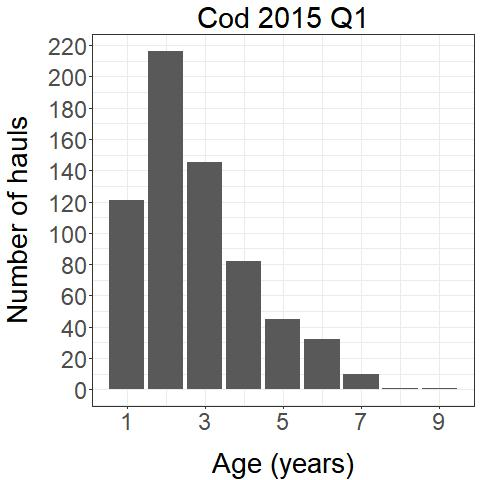
\includegraphics[width=0.28\textwidth]{figures/HaulsAndAge2015Q1Cod.jpeg}}
\qquad  
\subfloat[]{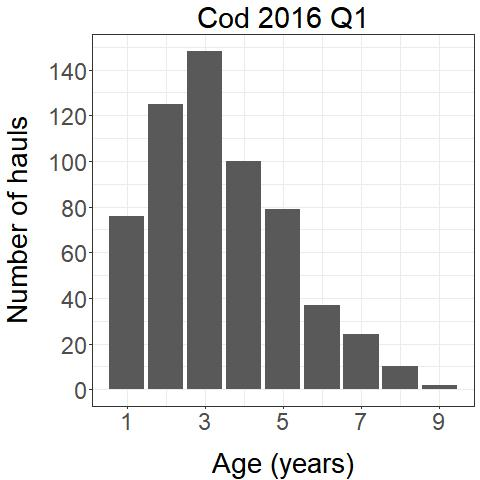
\includegraphics[width=0.28\textwidth]{figures/HaulsAndAge2016Q1Cod.jpeg}} 
\qquad
\subfloat[]{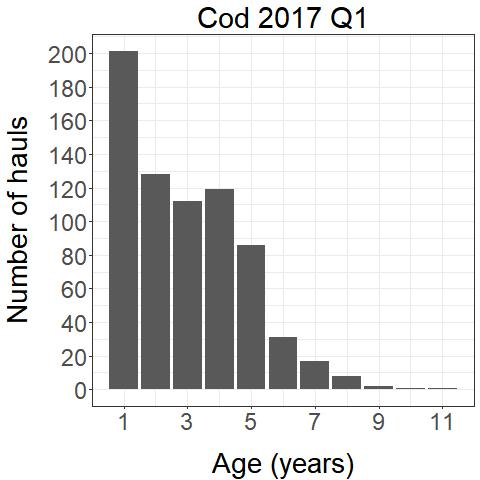
\includegraphics[width=0.28\textwidth]{figures/HaulsAndAge2017Q1Cod.jpeg}} \\
\qquad
\subfloat[]{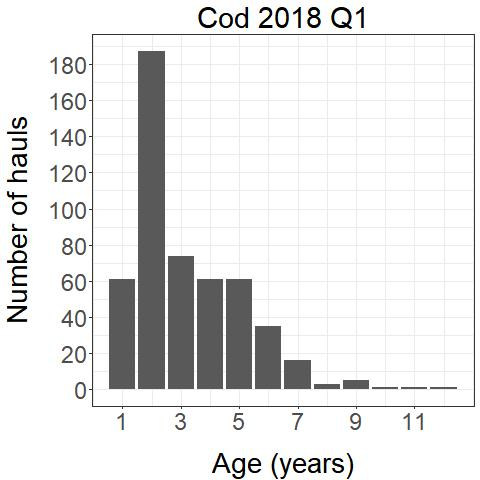
\includegraphics[width=0.28\textwidth]{figures/HaulsAndAge2018Q1Cod.jpeg}} 
\qquad 
\subfloat[ ]{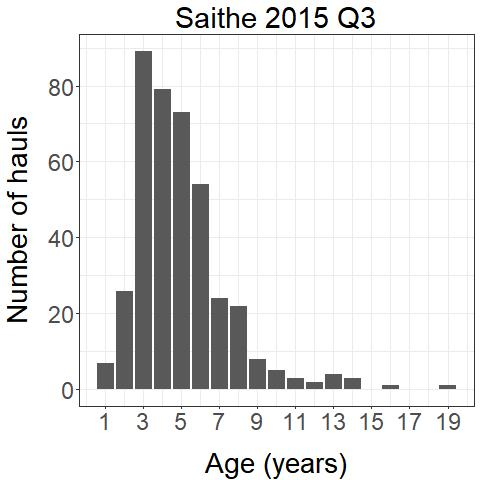
\includegraphics[width=0.28\textwidth]{figures/HaulsAndAge2015Q1Saithe.jpeg}} 
\qquad
\subfloat[ ]{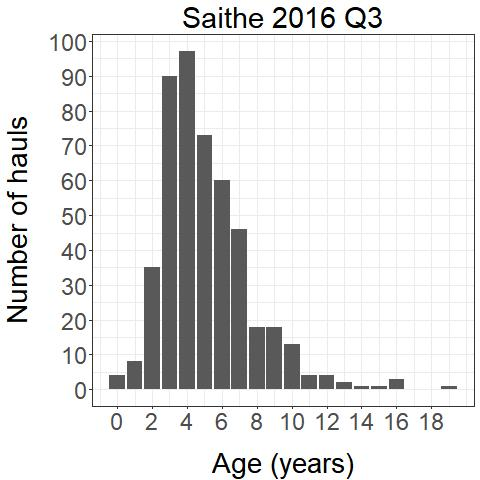
\includegraphics[width=0.28\textwidth]{figures/HaulsAndAge2016Q1Saithe.jpeg}} \\
\qquad
\subfloat[ ]{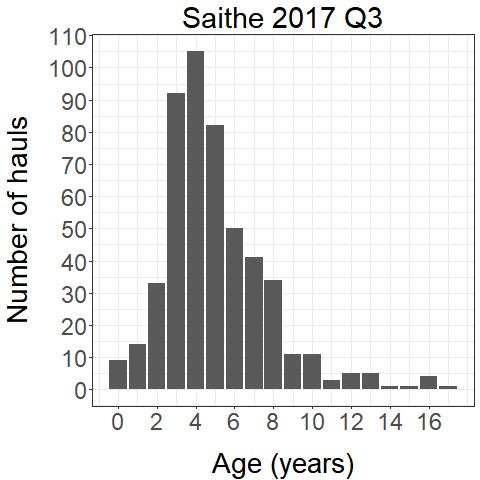
\includegraphics[width=0.28\textwidth]{figures/HaulsAndAge2017Q1Saithe.jpeg}}
\qquad
\subfloat[ ]{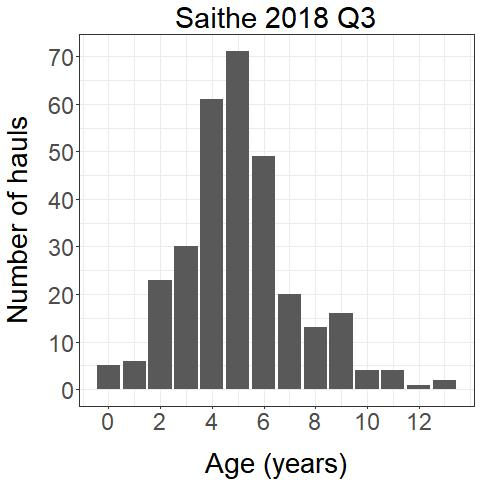
\includegraphics[width=0.28\textwidth]{figures/HaulsAndAge2018Q1Saithe.jpeg}} 
\end{tabular}
\captionsetup{font=small, width = 14.5cm}{
\caption[]{Number of hauls with age data for North Sea Cod and Saithe in quarters 1 an 3, respectively in the years 2015-2018. In Q3 surveys data is collected for age 0 group in the North Sea, however, no age 0 group data for Saithe were collected  in 2015 Q3.}
\label{HaulsAgeTotalAllYears}}
\end{figure*} 



\subsection{Evaluation of ALK methods}
\label{sec:codandsaitheresults}

Results from analyses of North Sea Cod  show that the area based ALK and haul based ALK estimators can give similar point estimates of abundance at age (Figure \ref{AreaHaulEstimatesAllYearsQ1}). The estimates are dominated by 2-year old in 2015, and by the 2 and 3-year olds in 2016. 
\begin{itemize}
\item uncertainty estimates for cohorts (juvenile Cod 1 and 2-year olds) in  2015-2016 does not correspond presumably because of 1) haul-to-haul variation in catch rates (see Figure \ref{AgeSCodALLYearsQ1} in Supplementary Materials \ref{secAP:realdataanalysis})?; 2) lower catch rates of 1-year old because who are typically not found in the North Sea during the winter but migrates to North Sea at age 2?
\item For Saithe, estimates of abundance at age from the two ALK estimators are rather different, particularly for 2, 3 or 4-year old in 2015-2016. Possible reasons for this?. Huge uncertainty captured in the 3-year old in 2016 Q3,which is not captured in 2-year old in 2015 Q3. Similarly in 2017 Q3 uncertainty in 1-year old is marginal, but this is huge in 2018 Q3 for the 2-year old.
\item  Estimates for Cod and Saithe quarters 3, and 1, respectively are given in Figure \ref{AreaHaulEstimatesAllYearsQ3} and \ref{AreaHaulEstimatesAllYearsQ3}, respectively in Supplementary Materials \ref{secAP:realdataanalysis}.
\end{itemize}
%The uncertainty in the 2-year olds in 2016 is quite large, which is not captured in 1-year olds in the previous year.


%\begin{itemize}
%\item Pool all hauls in a RFA, sample with replacement and put sampled hauls into relevant rectangles
%\item Sample with replacement the pooled age with a given length in a RFA




%\clearpage

\begin{figure*}[h!]
\centering
\begin{tabular}{@{}ccc@{}}
\subfloat[]{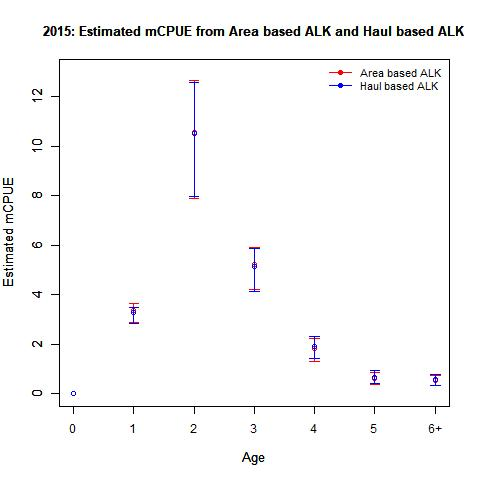
\includegraphics[width=0.4\textwidth]{figures/AreaHaulEstimates2015Q1.jpeg}} & 
\subfloat[ ]{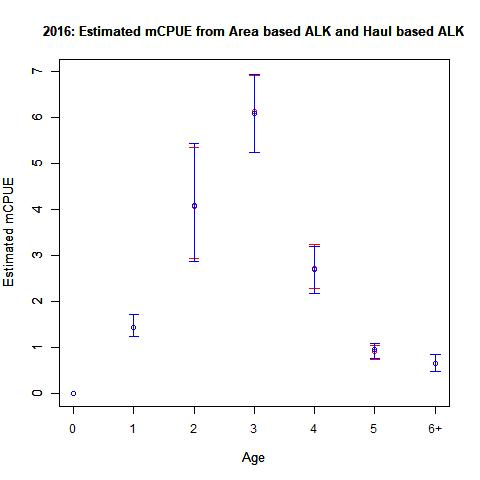
\includegraphics[width=0.4\textwidth]{figures/AreaHaulEstimates2016Q1.jpeg}} & \\
\subfloat[]{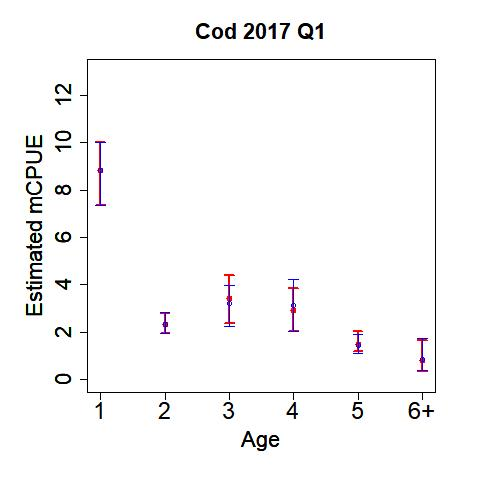
\includegraphics[width=0.4\textwidth]{figures/AreaHaulEstimates2017Q1.jpeg}} & 
\subfloat[]{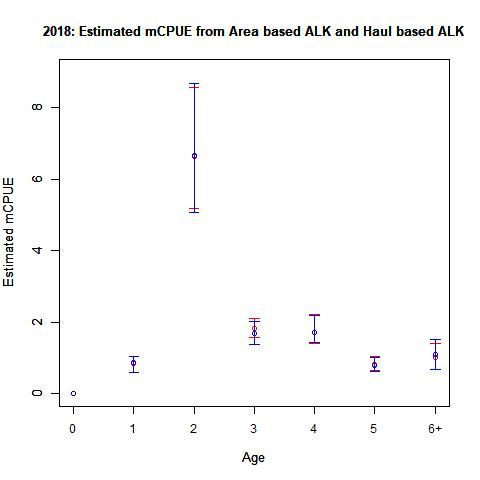
\includegraphics[width=0.4\textwidth]{figures/AreaHaulEstimates2018Q1.jpeg}} & 
\end{tabular}
\captionsetup{font=small, width = 14.5cm}{
\caption[]{Estimated abundance at age for North Sea Cod for the two ALK estimators based on data from the International Bottom Trawl Survey in 2015-2018 in the first quarter (Q1). The error bars are estimated 95\% confidence intervals using the bias corrected (see Methods) and 500 bootstrap samples. The age of Cod ranges from $1$ year to $6+$ years in the first quarter, where $6+$ is the "plus group consisting of all fish of age $6$ and older.  }\label{AreaHaulEstimatesAllYearsQ1}}
\end{figure*} 

\clearpage
\begin{figure*}[h!]
\centering
\begin{tabular}{@{}ccc@{}}
\subfloat[ ]{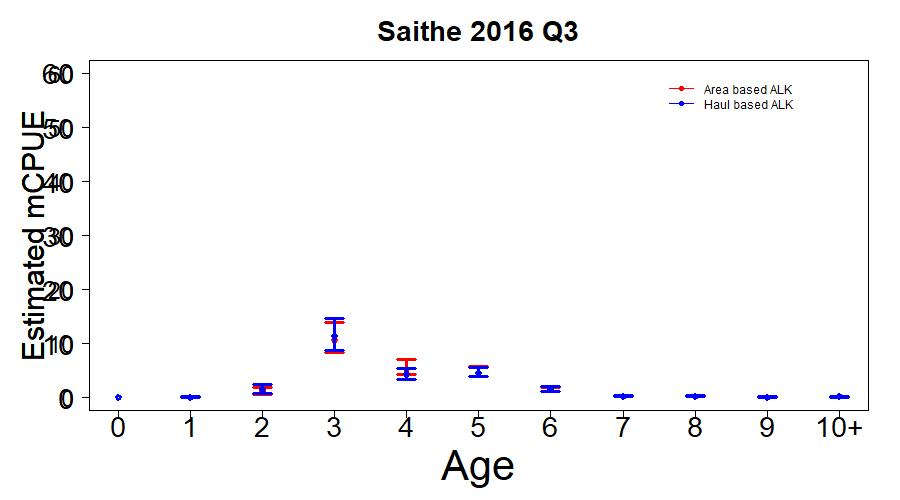
\includegraphics[width=0.4\textwidth]{figures/SaitheAreaHaulEstimates2015Q3.jpeg}} & 
\subfloat[ ]{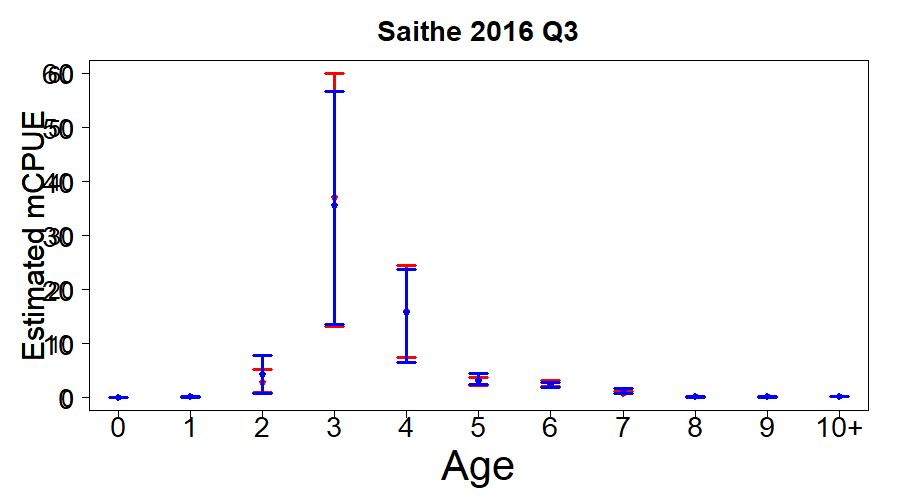
\includegraphics[width=0.4\textwidth]{figures/SaitheAreaHaulEstimates2016Q3.jpeg}} & \\
\subfloat[]{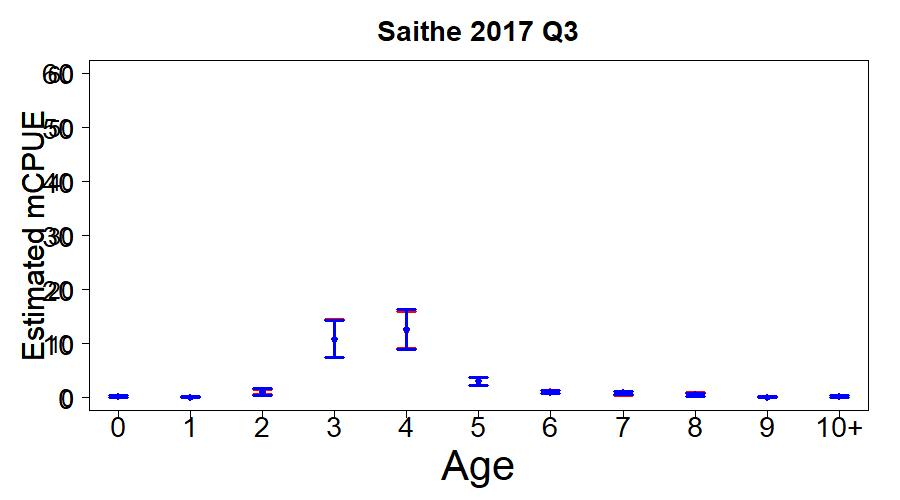
\includegraphics[width=0.4\textwidth]{figures/SaitheAreaHaulEstimates2017Q3.jpeg}} & 
\subfloat[]{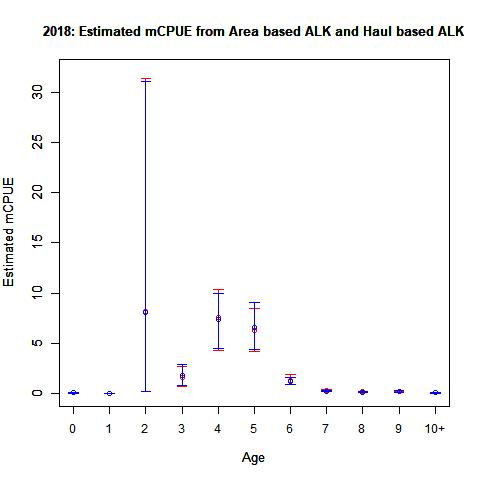
\includegraphics[width=0.4\textwidth]{figures/SaitheAreaHaulEstimates2018Q3.jpeg}} & 
\end{tabular}
\captionsetup{font=small, width = 14.5cm}{
\caption[]{Estimated abundance at age for North Sea Saithe for the two ALK estimators based on data from the International Bottom Trawl Survey in 2015-2018 in the third quarter (Q3). The error bars are estimated 95\% confidence intervals using the bias corrected (see Methods) and 500 bootstrap samples. The age of Saithe ranges from  $0$ year to $10+$ years in the third quarter, where $10+$ is the "plus group consisting of all fish of age $10$ and older.  }\label{SaitheAreaHaulEstimatesAllYearsQ3}}
\end{figure*} 


%\clearpage
\subsection{Comparison of bootstrap procedures for uncertainty estimation}
\begin{itemize}
\item stratified and modified-ICES boostrap procedures gave similar performances
\item ICES bootstrap procedure overestimates the uncertainty for both Cod and Saithe over the time series. This procedure ignores the fine scale stratification at the first stage, hence overestimation of the uncertainty; and gnores age-length data collected at the haul level, hence underestimates the uncertainty. So there is bias in both direction. 
\item Uncertainty in 2-year old Cod is typically higher compared with 1-year old even though 2-year olds were captured in at least 1.5 times more hauls than the 1-year olds in years 2015, 2016 and 2018 (Figure \ref{HaulsAgeTotalAllYears} (a) and (b)). The reason for this is because of the huge haul-to-haul variation in the catch rates;  see Figure \ref{AgeSCodALLYearsQ1} in Supplementary Materials \ref{secAP:realdataanalysis}.
\item Similarly for Saithe in the third quarter, uncertainty in the estimates of 2-year old is typical high, particularly in 2018. While 2-year old Saithe is caught in more hauls compared with 1-year olds (Figure \ref{HaulsAgeTotalAllYears} (h)), only one haul had approximately 36\% of the data, while the other hauls had at most 8\% of the data; see Figure \ref{AgeSaitheALLYearsQ3} (f) in Supplementary Materials \ref{secAP:realdataanalysis}.
\end{itemize}

%\clearpage
\begin{figure*}[h!]
\centering
\begin{tabular}{@{}ccc@{}}
\subfloat[]{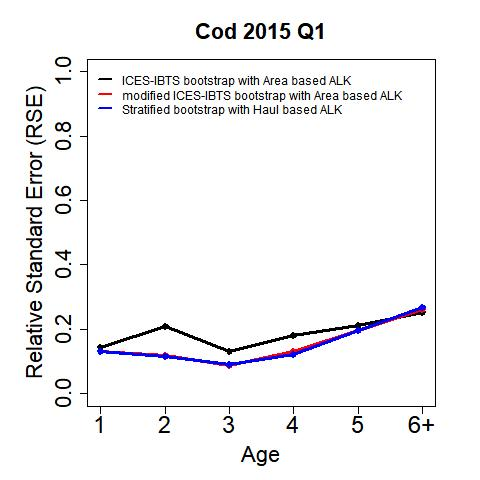
\includegraphics[width=0.4\textwidth]{figures/AreaHaulAreaMod2015Q1.jpeg}} & 
\subfloat[]{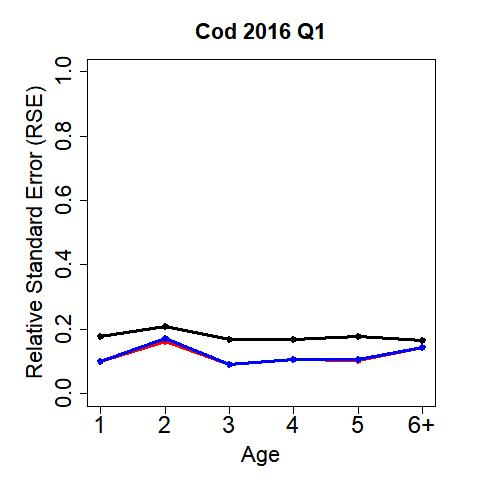
\includegraphics[width=0.4\textwidth]{figures/AreaHaulAreaMod2016Q1.jpeg}} & \\
\subfloat[]{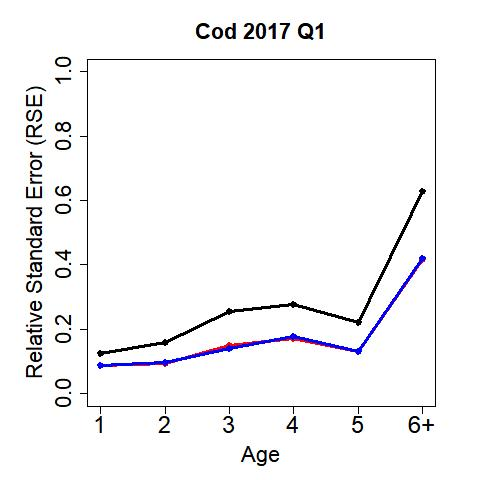
\includegraphics[width=0.4\textwidth]{figures/AreaHaulAreaMod2017Q1.jpeg}} & 
\subfloat[]{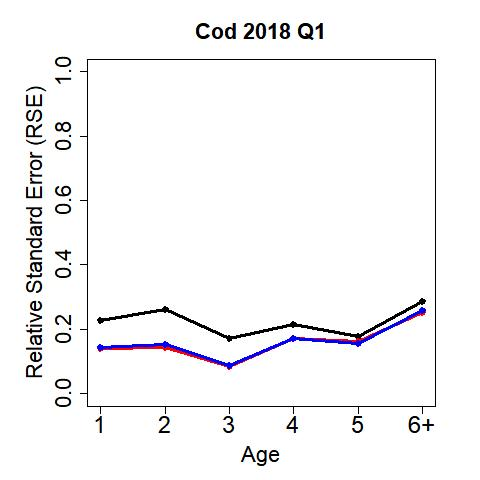
\includegraphics[width=0.4\textwidth]{figures/AreaHaulAreaMod2018Q1.jpeg}} & 
\end{tabular}
\captionsetup{font=small, width = 14.5cm}{
\caption[]{Expected relative standard error (RSE) for estimated abundance at age (mCPUE) for North Sea IBTS Cod in years 2015-2018 in the first quarter (Q1). The ICES-IBTS bootstrap procedure is compared with the modified ICES-IBTS and stratified bootstrap procedures. The ICES-IBTS bootstrap procedures are applied to the area based age-length key (ALK) and the stratified bootstrap procedure is applied to the haul based ALK. The age of Cod ranged from $1$ to $6+$ in the first quarter and $0$ year to $6+$ years in the third quarter, where $6+$ is the "plus group consisting of all fish of age $6$ and older.}}
\label{AreaAreaModAllYearsQ1}
\end{figure*} 



\clearpage

\begin{figure*}[h!]
\centering
\begin{tabular}{@{}ccc@{}}
\subfloat[]{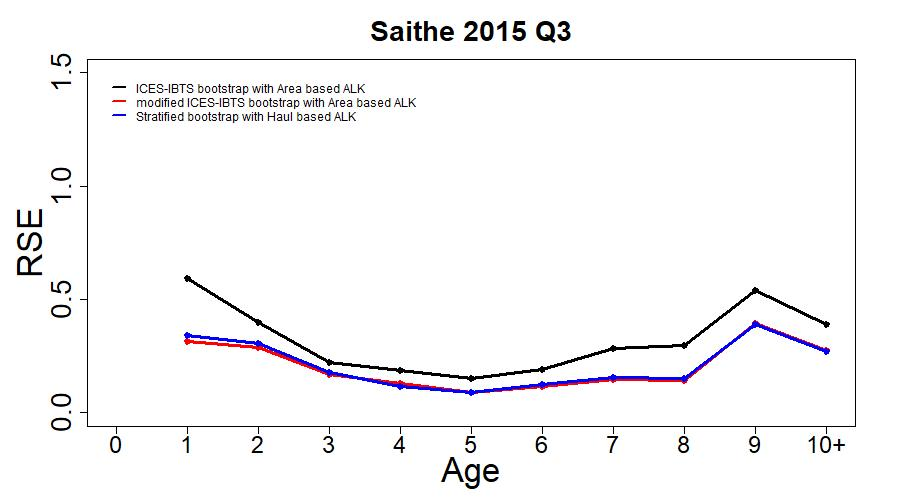
\includegraphics[width=0.4\textwidth]{figures/SaitheAreaHaulAreaMod2015Q3.jpeg}} & 
\subfloat[]{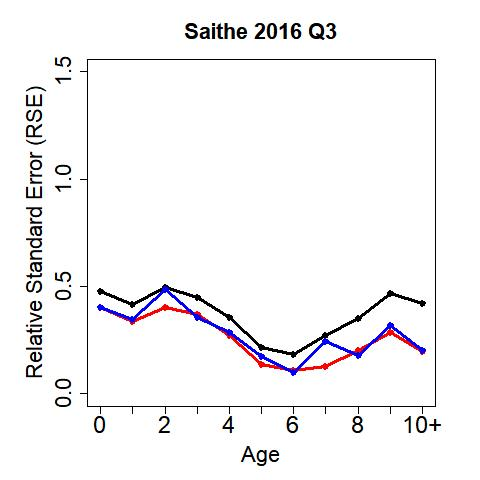
\includegraphics[width=0.4\textwidth]{figures/SaitheAreaHaulAreaMod2016Q3.jpeg}} & \\
\subfloat[]{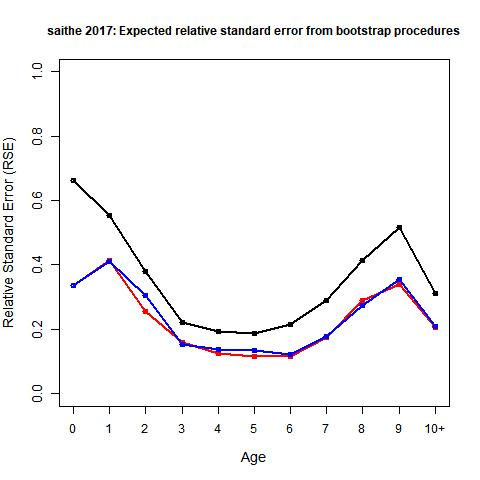
\includegraphics[width=0.4\textwidth]{figures/SaitheAreaHaulAreaMod2017Q3.jpeg}} & 
\subfloat[]{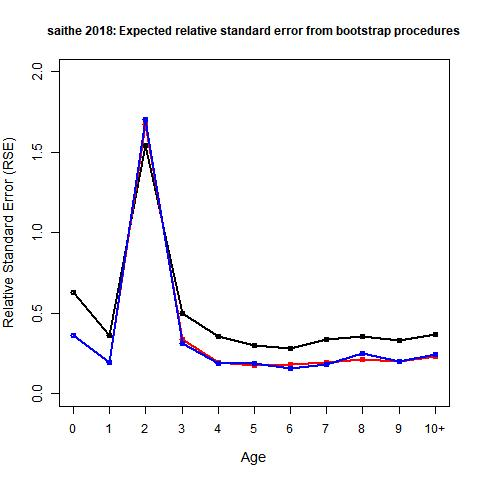
\includegraphics[width=0.4\textwidth]{figures/SaitheAreaHaulAreaMod2018Q3.jpeg}} & 
\end{tabular}
\captionsetup{font=small, width = 14.5cm}{
\caption[]{Expected relative standard error (RSE) for estimated abundance at age (mCPUE) for North Sea IBTS Saithe in years 2015-2018 in the third quarter (Q3). The ICES-IBTS bootstrap procedure is compared with the modified ICES-IBTS and stratified bootstrap procedures. The ICES-IBTS bootstrap procedures are applied to the area based age-length key (ALK) and the stratified bootstrap procedure is applied to the haul based ALK. The age of Saithe ranged from $1$ year to $10+$ years in the first quarter and $0$ to $10+$ in the third quarter, where $10+$ is the "plus group consisting of all fish of age $10$ and older.}}
\label{AreaAreaModAllYearsQ1}
\end{figure*} 




 \subsection{Comparison of the ALKs with an assessment study}
 In this section we compare the ALK procedures by investigating how the estimated spawning stock biomass (SSB) differs in an assessment study. We use the stock assessment model SAM \citep{nielsen2014estimation}, which is currently used in assessment for both the species in our case study. The default configurations in SAM are used. 
 
The estimated SSBs with usage of the two different ALKs are illustrated in Figure \ref{fig:assessment} for both Cod and Saithe. The differences in the estimated SSB between the two ALK procedures are marginal. Note that only the point estimates of the indices are used in the assessment study. Data needed for assessment, including the year range for the indices, are extracted from \href{www.stockassessment.org}{www.stockassessment.org}.  

\olav{(we should include the CV in the assessment modelling, and use the same configurations as in the real assessment (\ed{what are these configurations, explain or give example?}) --- \ed{use RSE-relative standard error instead of CV to be consistent in the paper?}---  \ed{perhaps we should be consistent with the years used in the paper (2015-2018)?})} 
 
 \begin{figure*}[h!]
\centering
\begin{tabular}{@{}ccc@{}}
\subfloat[]{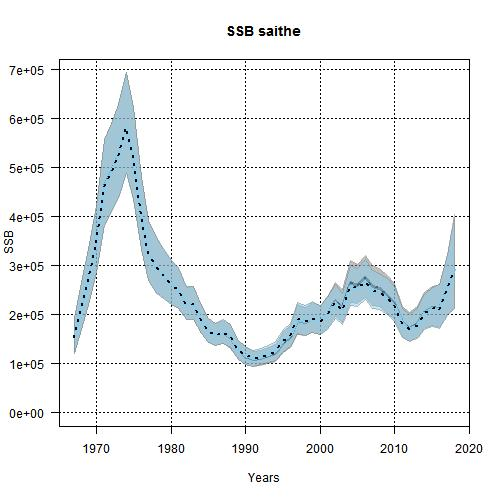
\includegraphics[width=0.45\textwidth]{figures/SAMsaitheSSB.jpeg}} & 
\subfloat[]{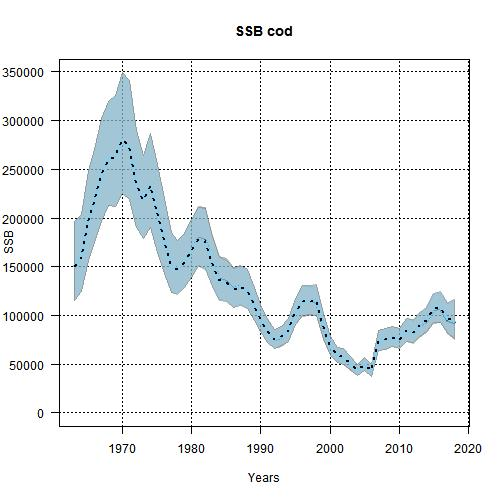
\includegraphics[width=0.45\textwidth]{figures/SAMCodSSB.jpeg}} & \\\end{tabular}
\captionsetup{font=small, width = 14.5cm}{
\caption[]{Estimated spawning stock biomass (SSB) with use of indices calculated with area based and haul based ALKs, with 95\% confidence intervals. The dotted lines and light blue intervals refers to assessment with use the haul based ALK. The dark line and grey interval refer to assessment with use of the area based ALK. }}
\label{fig:assessment}
\end{figure*} 


%\clearpage
\subsection{Evaluation of sampling strategy of otoliths}
\label{sec:optimumeffortresults}
In this section we investigate the effect of reducing effort with respect to otolith collection. The details of how the reduction is achieved are given in section \ref{sec:reducingeffort}.  We illustrate the effect by investigating how the relative standard error of the mCPUE (\ref{eq:abundanceestimatornorthsea}) changes, and how the spawning stock biomass changes in an assessment study. 

\subsection{Effect on the relative standard error}
Figure \ref{fig:removalCodQ1} illustrates the relative standard error (RSE) with several selections of length groups in year 2015-2018 Q1.  We see that the RSE typically increases as length group width increases. This increase seems to be particularly strong for Cod in age range 3-5 years. Compared to the original RSE, we see from Figure \ref{fig:removalCodQ1} that the RSE is almost unchanged when using twice as wide length groups below 40cm and the original length groups above 40cm.  At the same time, the number of sampled otoliths is typically reduce with approximately 30\% with that length group's selection (\ed{this is not very clear}). This observation gives a strong case for sampling fewer otoliths from short (and perhaps younger) fish as the effect on the mCPUE is minor. %(\ed{we should use relative standard error (RSE) instead of CV}).

%\clearpage
\begin{figure*}[h!]
\centering
\begin{tabular}{@{}ccc@{}}
\subfloat[]{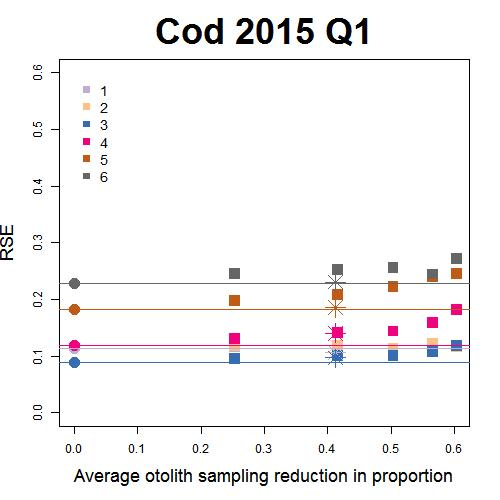
\includegraphics[width=0.45\textwidth]{figures/removalCod2015Q1.jpeg}} & 
\subfloat[]{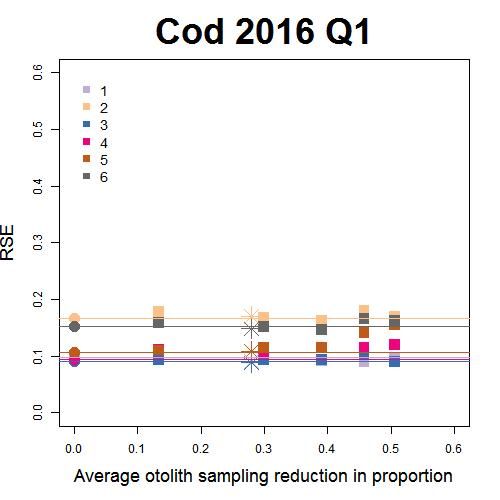
\includegraphics[width=0.45\textwidth]{figures/removalCod2016Q1.jpeg}} & \\
\subfloat[]{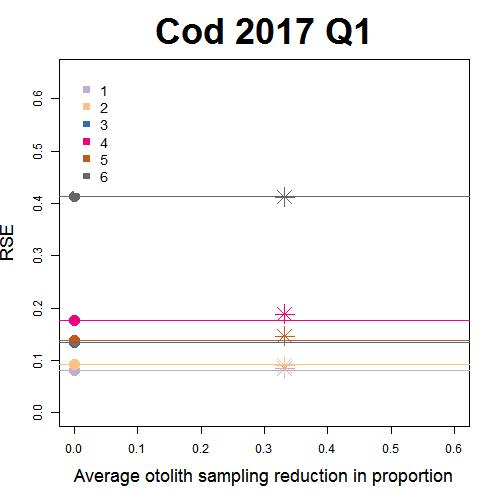
\includegraphics[width=0.45\textwidth]{figures/removalCod2017Q1.jpeg}} & 
\subfloat[]{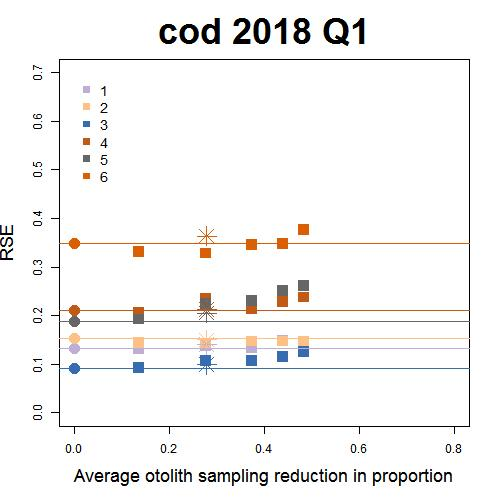
\includegraphics[width=0.45\textwidth]{figures/removalCod2018Q1.jpeg}} & 
\end{tabular}
\captionsetup{font=small, width = 14.5cm}{
\caption[]{Illustration of the CV for Cod in Q1 in year 2015-2018 with different length groups.  The squares illustrates CVs with use of length groups width 1cm, 2cm, ..., 5cm. The stars illustrates the CV with 2 cm length group width up to 40cm, and 1 cm above 40cm.  Only \textit{one} otolith is sampled inside each length group, and 200 bootstrap simulations are used. The horizontal lines illustrates the original CV with all data.}\label{fig:removalCodQ1}}
\end{figure*} 



\subsection{Effect on assessment}
\clearpage
\section{DISCUSSION}
\label{sec:discussion}

In this research we determine sufficient sampling efforts of otoliths for target species of the North Sea International Bottom Trawl Survey (IBTS). This is achieved by testing different sampling procedures that mimic the real data collection procedure but with a reduced number of otoliths. The estimated indices of abundance and their estimated uncertainty are investigated to determine if there is any real change in the precision of the estimates. Abundance indices are estimated using age-length keys (ALKs). The database for trawl surveys (DATRAS) manned by ICES includes an ALK that uses the raw proportions of age given length assuming constant age-length compositions over relatively large areas. We developed a haul based spatial ALK method  to estimate abundance indices and their variance that accounts for spatial variation in the data. 

%Figure \ref{fig:proportionRFA1CodQ1} illustrates the estimated age compositions as a function of length for a given haul in RFA 1. The haul selected is the haul with the most number of observed ages of Cod in 2018 Q1.

%
%\begin{figure}[h!]
%\centering
%\subfloat[]{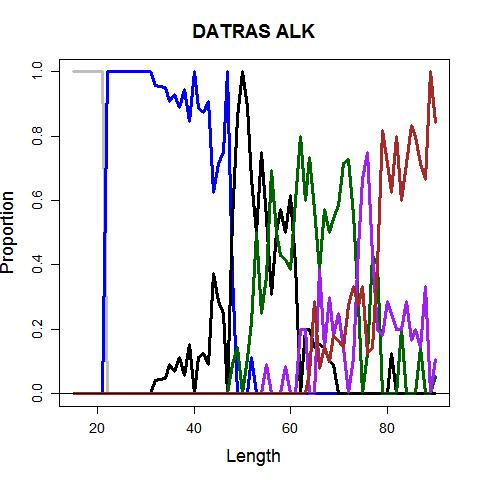
\includegraphics[scale=0.33]{figures/ALKdatrasQ1year2018RFA1.jpeg}}
%\subfloat[]{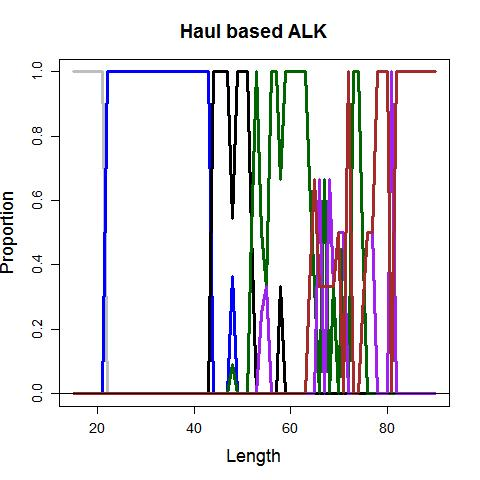
\includegraphics[scale=0.33]{figures/ALKhaulQ1year2018RFA1.jpeg}}
%%\subfloat[]{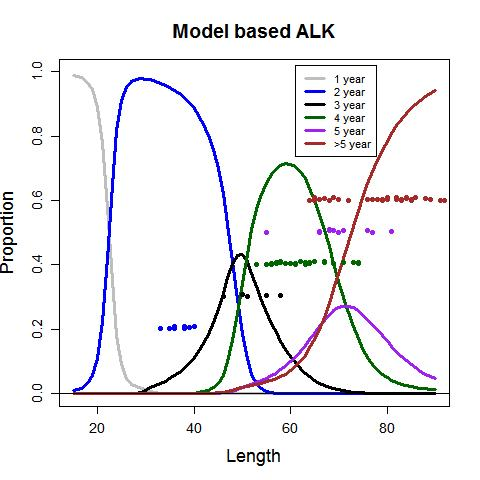
\includegraphics[scale=0.33]{figures/ALKmodelQ1year2018RFA1HaulWithMostObservations.jpeg}}
%\captionsetup{font=small, width = 14.5cm}{
% \caption{Estimated age compositions of Cod as a function of length in a given haul in RFA 1 using a) Area based ALK, b) haul based ALK. Note that explanation of the colours are only given in (b) (\ed{we need to give colurs here}). Each coloured point in (b) defines an observed Cod with the corresponding length and age in the haul. The haul selected is the haul with most observed ages of Cod in 2018 Q1. }\label{fig:proportionRFA1CodQ1}}
%\end{figure}



\clearpage








\clearpage

\bibliographystyle{apalike}
\bibliography{BibliographyIbts}

\clearpage


\begin{center}
\textbf{\Large Supplemental Materials: An Analysis of the North Sea International Bottom Trawl Survey.}
\end{center}
%%%%%%%%%% Merge with supplemental materials %%%%%%%%%%
%%%%%%%%%% Prefix a "S" to all equations, figures, tables and reset the counter %%%%%%%%%%
\setcounter{section}{0}
\setcounter{equation}{0}
\setcounter{figure}{0}
\setcounter{table}{0}
\setcounter{page}{1}
\makeatletter
\renewcommand{\thesection}{S\arabic{section}}
%\renewcommand{\theequation} {\arabic{section}. S\arabic{equation}}
%\renewcommand{\theequation}{S\arabic{equation}}
\renewcommand{\theequation}{S\arabic{section}.\arabic{equation}}
\renewcommand{\thefigure}{S\arabic{figure}}
\renewcommand{\bibnumfmt}[1]{[S#1]}
\renewcommand{\citenumfont}[1]{S#1}

\setcounter{table}{0}
\numberwithin{table}{section}
%\clearpage
\section{\large Areas fished by different countries in the North Sea IBTS}
\label{secAp:areasfishedappendix}
Typically, two countries fish each rectangle so that at least two trawl hauls are made per rectangle. However, intensified sampling is carried out in the following areas: at least 3 hauls per rectangle are taken in statistical rectangles  31F1, 31F2, 32F1, 33F4, 34F2, 34F3, 34F4, 35F3, 35F4; while six or more hauls per rectangle are taken in statistical rectangles  30F1, 32F2, 32F3, 33F2, 33F3 (ICES 1999).  The Skagerrak and Kattegat is fished solely by Sweden, who sample more than once in every rectangle while the west of Shetland (in Q1 and Q3) and inshore areas (Q3) is fished solely by Scotland. The edge of the Norwegian Trench is fished solely by Norway, but inshore areas near Denmark is fished by Denmark. The southern North Sea is fished by Denmark, Germany and England. France, typically, is the only country that surveys the western English Channel. Areas are surveyed by a single country because of the large proportion of untrawalable area (and subsequent gear damage issues experienced by other nations)  for efficient logistical purposes. Table \ref{countries} gives the countries and research vessels participating the North Sea IBTS.\\
\begin{small}
\begin{table}[h!]
\centering
\captionsetup{font=small, width = 15.5cm}{
\caption{Survey countries, vessel name, and period research vessels participating in first quarter (Q1) and third quarter (Q3) during 1997-2017.}\label{countries}}
\begin{tabular}{cccccccc}
\hline \\[0.1ex]
  & \multicolumn{2}{c}{\bf First Quarter (Q1)} & \multicolumn{2}{c}{\bf Third Quarter (Q3)}\\[1.5ex]
{\bf Country }  & Vessel name & Period    & Vessel name & Period  \\[0.5ex]
\hline \\[0.5ex]
Denmark  &   Dana   &   January-February  & Dana & July-August    \\[1ex]
France  & Thalassa II & January-February & - & -   \\[1ex]
Germany   &  Walther  Herwig III & January-February   &   Walther  Herwig III & July-August \\[1ex]
Netherlands &  Tridens 2 &  January-February   & - & -     \\[1ex]
Norway  &   G.O. Sars  & January-February &    Johan Hjort  & July   \\[1ex]
UK England &- & -&  Endeavour &  August-September  \\[1ex]
UK Scotland   &  Scotia III &  January-February & Scotia III &  July-August \\[1ex]
Sweden  &  Dana &  January-February  &  Dana &  August                  \\[0.5ex]
\hline
\end{tabular}
\end{table}
\end{small}




%\clearpage
\section{\large Otolith sampling per fish species}
\label{secAp:otolithappendix}
From 1991-2017, most countries conducted quota sampling of otoliths per length group in a RFA. But from 2013, Norwa, Scotland and the Netherlands have been sampling one otolith per length class from each trawl haul. From 2018 Q1, all countries are required to sample one otolith per length class per trawl haul.  Table \ref{tab:otolithsTable} gives the minimum sampling levels of otoliths for the target species.\\ %However, for the smallest size groups, that presumably contain only one age group, the number of otoliths per length class may be reduced, and more otoliths per length are required for the larger length classes.\\ %\\
%\clearpage
\begin{small}
\begin{table}[h!]
\centering
\caption{Minimum sampling levels of otoliths by species for RFA or per trawl haul.}
\label{tab:otolithsTable}
\begin{tabularx}{\linewidth}{r l l l l X}
\toprule 
Period &  Species  & Minimum sampling levels of otoliths per length class    \\[0.7ex]
\midrule \\[0.1ex]
{\bf 1991-2017} & & {\bf Number of otoliths per length class in a RFA}  \\[1.0ex]
     & herring  &  $8$  otoliths per $\frac{1}{2}$ cm group \\[0.5ex]
     & sprat    & $16$  otoliths per $\frac{1}{2}$ cm length class  $8.0 -11.0$ cm\\[0.5ex]
              & & $12$  otoliths per $\frac{1}{2}$ cm length class  $\geq 11.0$ cm\\[0.5ex]
& mackerel      & $8$  otoliths per $\frac{1}{2}$ cm length class \\[0.5ex]
& Cod       	  & $8$  otoliths per $1$ cm length class\\[0.5ex]
&haddock   	  & $8$  otoliths per $1$ cm length class \\[0.5ex]
&whiting    	  & $8$  otoliths per $1$ cm length class \\[0.5ex]
&Norway pout   & $8$  otoliths per $1$ cm length class\\[0.5ex]
&Saithe        & $8$  otoliths per $1$ cm length class \\[1ex] 
& All target species      &  From 2013 Norway and Scotland, and  Netherlands from 2016 \\[0.7ex] 
&& have been sampling 1 otolith per length class from each trawl haul \\[0.7ex] 
&& (to 0.1$\cm$ below for shellfish, to 0.5$\cm$ below for herring and sprat, and \\ [0.7ex] 
&& to 1$\cm$ below for all other species).\\[1.7ex] 

{\bf 2018} & & {\bf Number of otoliths per length class per trawl haul}  \\[1.0ex]
  & herring  &  $1$  otolith per $\frac{1}{2}$ cm group \\[0.5ex]
     & sprat    & $1$  otolith per $\frac{1}{2}$ cm length class  $8.0 -11.0$ cm\\[0.5ex]
              & & $1$  otolith per $\frac{1}{2}$ cm length class  $\geq 11.0$ cm\\[0.5ex]
& mackerel      & $1$  otolith per $1$ cm length class \\[0.5ex]
& Cod       	  & $1$  otolith per $1$ cm length class\\[0.5ex]
& haddock & $2$  otoliths per $5$ cm length class $11 -15, \ 16-20, \ 21-25, \ 26-30$ cm \\[0.5ex]
& Norway pout & $2$  otoliths per $5$ cm length class $5 -10, \ 11-15$ cm\\[0.5ex]
               & & $2$  otoliths per $1$ cm length class $> 15$ cm\\[1.0ex]
&Saithe        & $1$  otolith per $1$ cm length class \\[0.5ex]  
&plaice       & $1$  otolith per $1$ cm length class \\[0.1ex]
\bottomrule         
\end{tabularx}
\end{table}
\end{small}


\section{Pseudo bootstrap method}
\label{secAp:pseudobootstrap}
Assume a length $l$ group has $n_{l}$ sub length groups. Assume further in a given haul and a length group that the vector of number of observed lengths and ages within each sub length group are ${\bf x} = \left(x_{1},...,x_{nl}\right)$ and ${\bf a} = \left(a_{1},...,a_{nl}\right)$.  The pseudo bootstrap procedure is defined as follows:

\begin{enumerate}
\item For a given length group, do the following for each sub length group, $i$, inside the length group: Define $k$ as the largest value such that $ka_{i} \leq x_{i}$. Sample without replacement $x_{i} - k a_{i}$ observed ages in the given haul and the given sub length group, and denote these samples as $a^{\mathrm{extra}}_{i}$. Define the pseudo population of age observation in sub length group $i$, $a^{(s)*}_{i}$, as the union of $k$ replications of the observed ages in the sub length group and $a^{\mathrm{extra}}_{i}$.

\item Define $a^{*}_{l} = \cup_{i = 1}^{n_{l}} a^{(s)*}_{i} $, where $a^{(s)*}_{i}, \ i \in \left(1,...,n_{l} \right)$, are the pseudo populations obtained in step 2.

\item Sample without replacement $\sum_{i = 1}^{n_{l}} a_{i}$ samples from $a^{*}_{l} $.

\item Repeat steps $2-4$ for each haul and length group.
\end{enumerate}

\clearpage
\section{\large IBTS data set for Cod and Saithe}
\label{secAp:data}

%Table \ref{tab:realdata2017-2018} describes the data for the years 2015-2018.

%\clearpage
 \begin{small}
\begin{table}[h!]
\setlength\tabcolsep{3.5pt} 
\centering
\captionsetup{font=small, width = 15cm}{
\caption{Summary of North Sea Cod and Saithe data in years 2015-2018.  Data collected in the third quarter (Q3) has age 0 group but this is not collected in quarter 1 (Q1) surveys.}\label{tab:realdata2017-2018}}
\begin{footnotesize}
\begin{tabular}{clclclclclclclclclclclclclclclclclclclclclclclclclclclclclclclclclcl}
  \hline \\ [0.3ex]
{\bf Species} &  & \multicolumn{8}{c}{\bf Years and quarters} &   \\[1.0ex]
%\hline\\
%  \cmidrule(lr{0.3em}){3-6} \\ [0.5ex]% \cmidrule(lr{0.3em}){5-6}  \\ [0.5ex]
&  & \multicolumn{2}{c}{2015} & \multicolumn{2}{c}{2016}  & \multicolumn{2}{c}{2017} & \multicolumn{2}{c}{2018}   \\ [1.0ex]
 \hline \\ [0.3ex]
& & Q1  & Q3 & Q1  & Q3 & Q1  & Q3 & Q1  & Q3 & \\
%\hline \\ 
  \cmidrule(lr{0.3em}){3-10}  \\ [0.5ex]% \cmidrule(lr{0.3em}){13-20}  \\ [0.5ex]
 	& Number of hauls   & 380 & 352 & 360 & 381 &377 & 337 & 372 &349   \\ [1.0ex]
 	& Mean time of hauls (in minutes) & 28.55 & 23.44 & 28.40 & 22.47 &29.02 & 29.37 &  29.26 & 29.13 \\ [1.2ex]
\raisebox{2.5ex}{\bf Cod}        \\ %   & Trawls &   &  &   & & &               & & 345 & 372 &   \\ [1.5ex]
& Age range (in years)               & 1 - 9 & 0 - 8 & 1 - 10 & 0 - 10 & 1 - 11 & 0 - 11  &  1 - 12 & 0 - 11\\ [1.2ex]
%& Length range (in cm)               & 9 - 113 &7 - 111 &11 - 109 & 5 - 110 & 7 - 115 & 6 - 112 &  11 - 114 & 5 - 107  \\[1.5ex] 
& Total otoliths sampled for age determination               & 2895 &2113 & 2046 & 1804    &2501 & 2230  & 1600 & 1456 \\[1.2ex] 
& Number of hauls with length data & 305 &216 & 251 & 230& 306 & 237  & 237 & 199 \\[1.2ex]
& Number of hauls with age data    & 301 &209 & 243 & 224 & 293 & 236 & 229 & 195 \\[1.2ex]
& Cod with missing age in RFAs     & 0.30\%& 0.13\% & 0.13\% & 0.34\% & 0.68\% &  0.07\% & 0.51\%  & 0.11\%  \\[1.2ex]  
& Cod with missing age in hauls    & 10.06\% & 14.20\% & 6.18\%& 6.32\% & 2.25\% &0.27\%   & 1.40\%   & 0.77\% \\[2.2ex] 


\raisebox{2.5ex}{\bf Saithe}        \\
& Age range (in years)                         &1 - 16   & 0 - 19 &1 - 17   &0 - 19 &1 - 15 & 0 - 11 &  1 - 12 & 0 - 13 \\ [1.2ex]
& Total otoliths sampled for age determination & 600  & 1526 & 581  &1631 &1083 & 2163  & 822 & 1085\\[1.2ex] 
%& Length range (in cm)           & 13 - 110  & 21 - 109 & 16 - 107  & 12 - 115  &15 - 108 & 6 - 112 &  11 - 114 & 7 - 109     &  \\[1.5ex] 
& Number of hauls with length data & 73 &117 &97 & 135& 122& 128  & 83 & 98\\[1.2ex]
& Number of hauls with age data    & 71 &116 & 74& 132 & 111& 127 & 81 & 97\\[1.2ex]
& Saithe with missing age in RFAs      &1.2\% & 0\%		& 0\%  & 0.03\% &0.14\%  &  0.05\% & 0.03\%  & 0\%  \\[1.2ex]  
& Saithe with missing age in hauls     &21.6\%& 0.17\%	& 0.4\%&0.22\%  &20.1\%  &   0.08\% & 0.06\%  & 0.02\%  \\[0.5ex]

   \hline \\[0.1ex]
\end{tabular}
\end{footnotesize}
\end{table}
 \end{small}
 
 
%\clearpage
\section{Real data analysis}
\label{secAP:realdataanalysis}
In this Section we give results for Cod in the third quarter (Q3) and for Saithe in the first quarter (Q1)  in years 2015-2018. Section \ref{secAp:comparisonOfALK} compares the ALK estimators used to compute abundance at age indices of Cod and Saithe. In Section \ref{secAP:uncertaintyBootstrapMethods}, we compare the relative standard error of abundance at age from the  three bootstrap procedures. Figures \ref{AgeSCodALLYearsQ1} and \ref{AgeSaitheALLYearsQ3} give the  number of North Sea juvenile Cod and Saithe, respectively, sampled in years 2015, 2016 and 2018. Haul-to-haul variation in catch rates of 2-year old Cod is much higher compared with 1-year old Cod in 2016 and 2018. Similarly for Saithe in Q3, haul-to-haul variation is high for 2-year olds in 2016 and 2018 compared with 1-year olds (Figure \ref{AgeSaitheALLYearsQ3}).

\clearpage
\begin{figure*}[h!]
\centering
\begin{tabular}{@{}ccc@{}}
\subfloat[Saithe in year 2018 Q3]{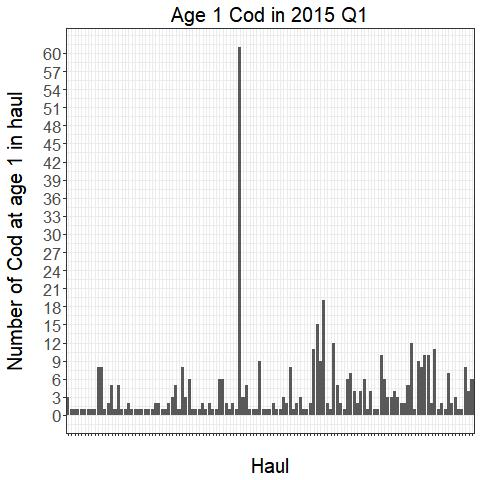
\includegraphics[width=0.4\textwidth]{figures/Age1Cod2015Q1.jpeg}}
\qquad
\subfloat[]{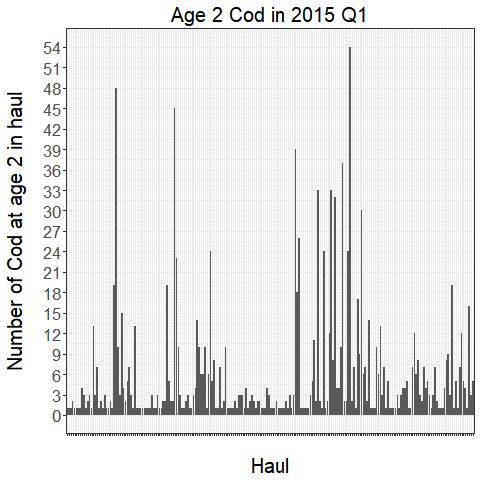
\includegraphics[width=0.4\textwidth]{figures/Age2Cod2015Q1.jpeg}} \\
\qquad 
\subfloat[]{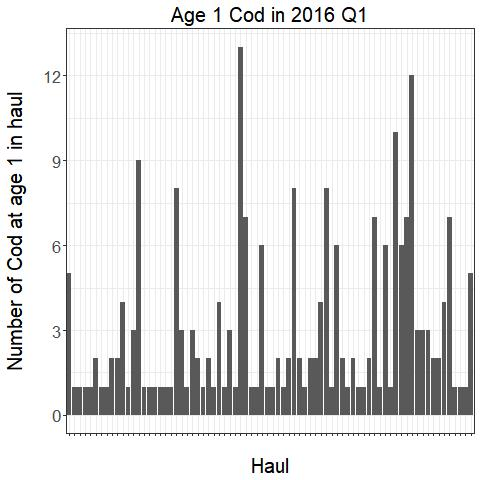
\includegraphics[width=0.4\textwidth]{figures/Age1Cod2016Q1.jpeg}}  
\qquad
\subfloat[]{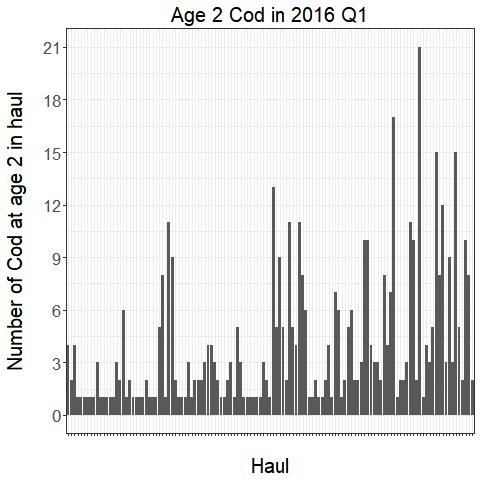
\includegraphics[width=0.4\textwidth]{figures/Age2Cod2016Q1.jpeg}}  \\
\qquad
\subfloat[]{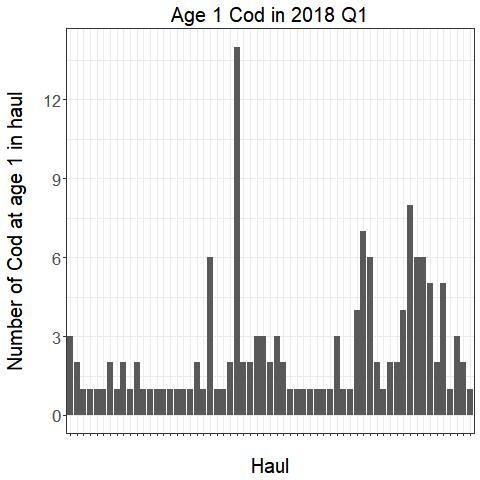
\includegraphics[width=0.4\textwidth]{figures/Age1Cod2018Q1.jpeg}}  
\qquad
\subfloat[]{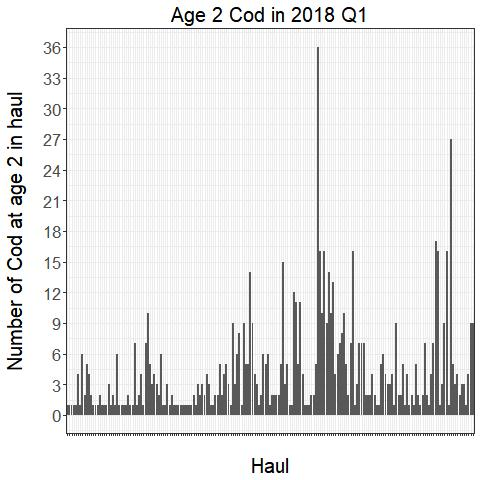
\includegraphics[width=0.4\textwidth]{figures/Age2Cod2018Q1.jpeg}}  
\end{tabular}
\captionsetup{font=small, width = 14.5cm}{
\caption[]{The number of age 1 and 2-year old Cod sampled in hauls in 2015, 2016 and 2018.   }\label{AgeSCodALLYearsQ1}}
\end{figure*} 


\clearpage
\begin{figure*}[h!]
\centering
\begin{tabular}{@{}ccc@{}}
\subfloat[]{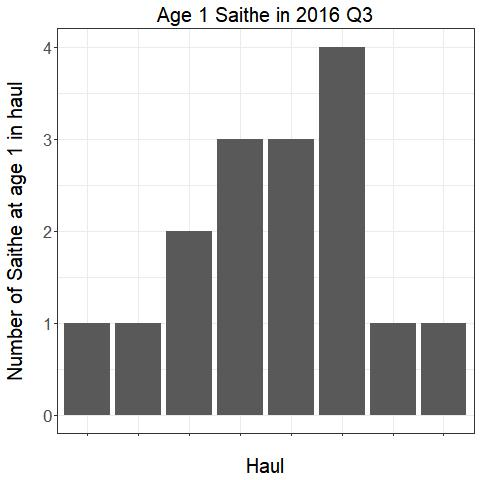
\includegraphics[width=0.4\textwidth]{figures/Age1Saithe2016Q3.jpeg}} 
\qquad
\subfloat[]{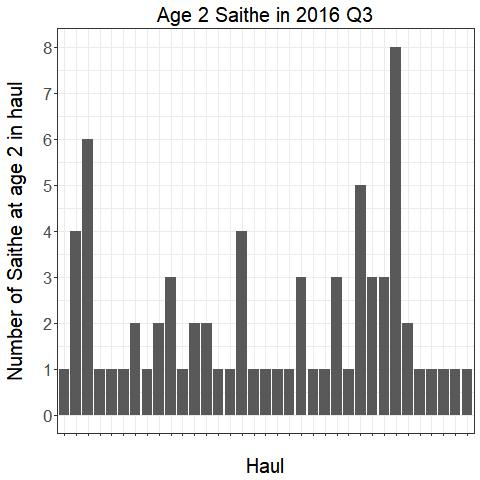
\includegraphics[width=0.4\textwidth]{figures/Age2Saithe2016Q3.jpeg}} \\
\qquad 
\subfloat[]{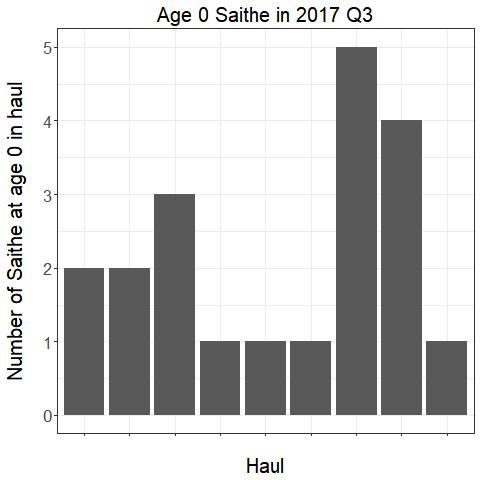
\includegraphics[width=0.4\textwidth]{figures/Age0Saithe2017Q3.jpeg}}  
\qquad 
\subfloat[]{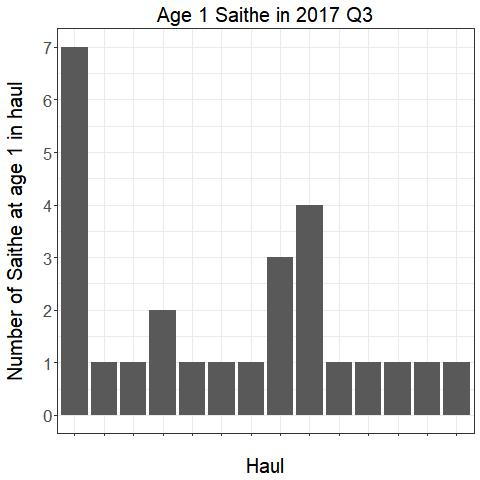
\includegraphics[width=0.4\textwidth]{figures/Age1Saithe2017Q3.jpeg}}  \\
\qquad
\subfloat[]{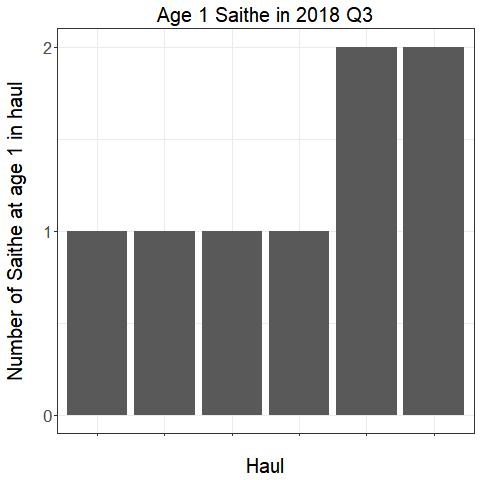
\includegraphics[width=0.4\textwidth]{figures/Age1Saithe2018Q3.jpeg}}  
\qquad 
\subfloat[]{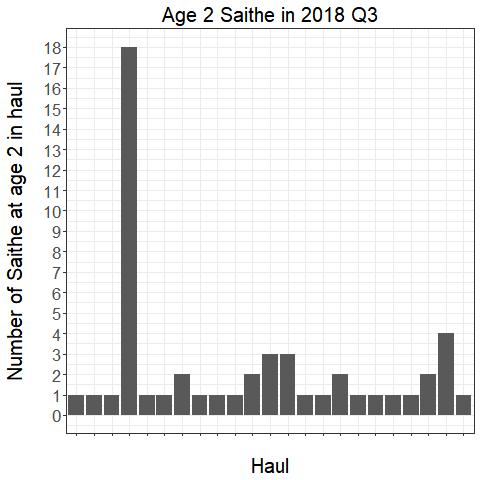
\includegraphics[width=0.4\textwidth]{figures/Age2Saithe2018Q3.jpeg}}  
\end{tabular}
\captionsetup{font=small, width = 14.5cm}{
\caption[]{The number of age 0, 1 and 2-year old Saithe sampled in hauls in 2016-2018.  }\label{AgeSaitheALLYearsQ3}}
\end{figure*} 

%Approximately 65.22\% of hauls had one sample of age 2, and 4.35 \% had 18 observations, while approximately 17.39 \% had two observations, 8.7\% had 3 observations and 4.35\% had 4 observations. For age 0
 
\clearpage
\subsection{Comparison of ALK methods for North Sea Cod and Saithe}
\label{secAp:comparisonOfALK}
The results show that the two ALK estimators can give similar estimates of abundance at age of Cod in all years (Figure \ref{AreaHaulEstimatesAllYearsQ3}). In years 2015-2017, the estimates are dominated by juvenile Cod (0 and 1-year olds). For Saithe, however, the estimated abundance at age from the two ALK methods are rather different, particularly for fish between ages 3 - 6 years (Figure \ref{SaitheAreaHaulEstimatesAllYearsQ1}). The differences in point estimates can be explained by the .....

%\clearpage

\begin{figure*}[h!]
\centering
\begin{tabular}{@{}ccc@{}}
\subfloat[]{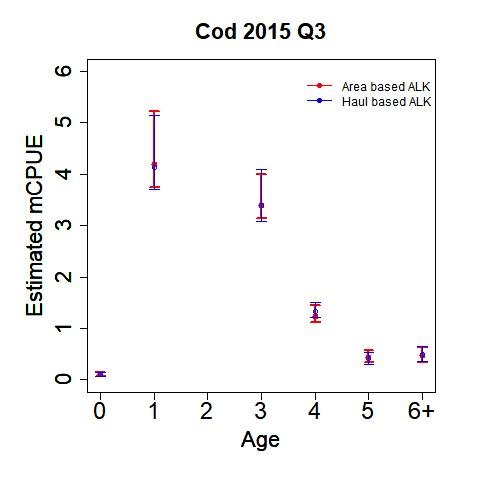
\includegraphics[width=0.4\textwidth]{figures/AreaHaulEstimates2015Q3.jpeg}} & 
\subfloat[]{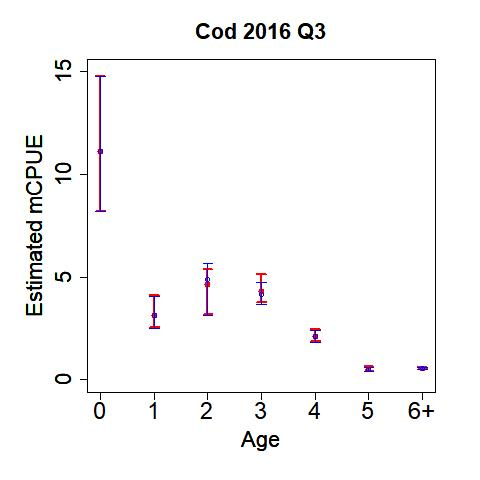
\includegraphics[width=0.4\textwidth]{figures/AreaHaulEstimates2016Q3.jpeg}} & \\
\subfloat[]{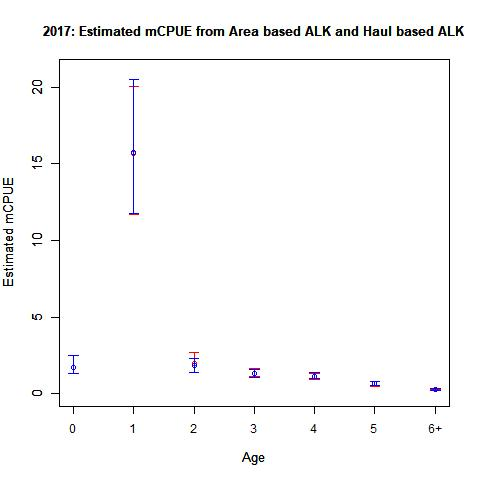
\includegraphics[width=0.4\textwidth]{figures/AreaHaulEstimates2017Q3.jpeg}} & 
\subfloat[]{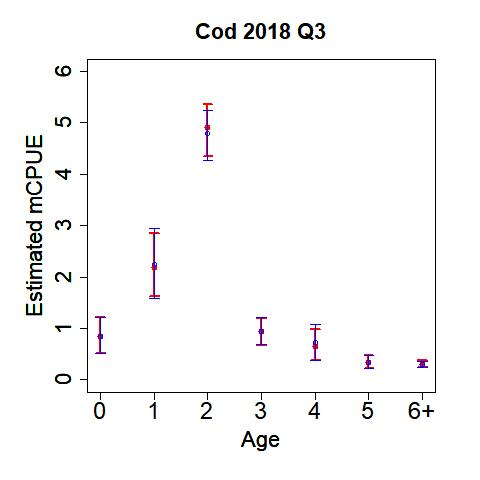
\includegraphics[width=0.4\textwidth]{figures/AreaHaulEstimates2018Q3.jpeg}} & 
\end{tabular}
\caption[]{Estimated abundance at age of North Sea Cod by the area based ALK and haul based ALK estimators based on data from the International Bottom Trawl Survey in 2015-2018 in the first quarter (Q1). The error bars are estimated 95\% confidence intervals using the bias corrected (see Methods) and 500 bootstrap samples. The age of Cod ranges from $1$ year to $10+$ years, where $6+$ is the "plus group consisting of all fish of age $6$ and older.  }
\label{AreaHaulEstimatesAllYearsQ3}
\end{figure*} 


\clearpage
\begin{figure*}[h!]
\centering
\begin{tabular}{@{}ccc@{}}
\subfloat[]{\includegraphics[width=0.4\textwidth]{figures/SaitheAreaHaulEstimates2015Q1.jpeg}} & 
\subfloat[ ]{\includegraphics[width=0.4\textwidth]{figures/SaitheAreaHaulEstimates2016Q1.jpeg}} & \\
\subfloat[]{\includegraphics[width=0.4\textwidth]{figures/SaitheAreaHaulEstimates2017Q1.jpeg}} & 
\subfloat[]{\includegraphics[width=0.4\textwidth]{figures/SaitheAreaHaulEstimates2018Q1.jpeg}} & 
\end{tabular}
\caption[]{Estimated abundance at age of North Sea Saithe by the area based ALK and haul based ALK estimators based on data from the International Bottom Trawl Survey in 2015-2018 in the first quarter (Q1). The error bars are estimated 95\% confidence intervals using the bias corrected (see Methods) and 500 bootstrap samples. The age of Saithe ranges from $1$ year to $10+$ years, where $10+$ is the "plus group consisting of all fish of age $10$ and older.  }
\label{SaitheAreaHaulEstimatesAllYearsQ1}
\end{figure*} 
 
\clearpage
\subsection{Comparing bootstrap methods}
\label{secAP:uncertaintyBootstrapMethods}


\begin{figure*}[h!]
\centering
\begin{tabular}{@{}ccc@{}}
\subfloat[]{\includegraphics[width=0.4\textwidth]{figures/AreaHaulAreaMod2015Q3.jpeg}} & 
\subfloat[]{\includegraphics[width=0.4\textwidth]{figures/AreaHaulAreaMod2016Q3.jpeg}} & \\
\subfloat[]{\includegraphics[width=0.4\textwidth]{figures/AreaHaulAreaMod2017Q3.jpeg}} & 
\subfloat[]{\includegraphics[width=0.4\textwidth]{figures/AreaHaulAreaMod2018Q3.jpeg}} & 
\end{tabular}
\caption[]{Expected relative standard error (RSE) for estimated abundance at age (mCPUE) for North Sea IBTS Cod in years 2015-2018 in the third quarter (Q3). The ICES-IBTS bootstrap procedure is compared with the modified ICES-IBTS and stratified bootstrap procedures for 500 replicates. The ICES-IBTS bootstrap procedures are applied to the area based age-length key (ALK) and the stratified bootstrap procedure is applied to the haul based ALK. The age of Cod ranges $0$ year to $6+$ years in the third quarter, where $6+$ is the "plus group consisting of all fish of age $6$ and older.}
\label{AreaAreaModAllYearsQ3}
\end{figure*} 

\clearpage

\begin{figure*}[h!]
\centering
\begin{tabular}{@{}ccc@{}}
\subfloat[]{\includegraphics[width=0.4\textwidth]{figures/SaitheAreaHaulAreaMod2015Q1.jpeg}} & 
\subfloat[]{\includegraphics[width=0.4\textwidth]{figures/SaitheAreaHaulAreaMod2016Q1.jpeg}} & \\
\subfloat[]{\includegraphics[width=0.4\textwidth]{figures/SaitheAreaHaulAreaMod2017Q1.jpeg}} & 
\subfloat[]{\includegraphics[width=0.4\textwidth]{figures/SaitheAreaHaulAreaMod2018Q1.jpeg}} & 
\end{tabular}
\caption[]{Expected relative standard error (RSE) for estimated abundance at age (mCPUE) for North Sea IBTS Saithe in years 2015-2018 in the first quarter (Q1). The ICES-IBTS bootstrap procedure is compared with the modified ICES-IBTS and stratified bootstrap procedures. The ICES-IBTS bootstrap procedures are applied to the area based age-length key (ALK) and the stratified bootstrap procedure is applied to the haul based ALK. The age of Saithe ranges from $1$ year to $10+$ years in the first quarter, where $10+$ is the "plus group consisting of all fish of age $10$ and older.}
\label{AreaAreaModAllYearsQ1}
\end{figure*} 

\end{document}